%%%%%%%%%%%%%%%%%%%%%%%%%%%%%%%%%%%%%%%%%
% Masters/Doctoral Thesis 
% LaTeX Template
% Version 2.5 (27/8/17)
%
% This template was downloaded from:
% http://www.LaTeXTemplates.com
%
% Version 2.x major modifications by:
% Vel (vel@latextemplates.com)
%
% This template is based on a template by:
% Steve Gunn (http://users.ecs.soton.ac.uk/srg/softwaretools/document/templates/)
% Sunil Patel (http://www.sunilpatel.co.uk/thesis-template/)
%
% Template license:
% CC BY-NC-SA 3.0 (http://creativecommons.org/licenses/by-nc-sa/3.0/)
%
%%%%%%%%%%%%%%%%%%%%%%%%%%%%%%%%%%%%%%%%%

%%%%%%%%%%%%%%%%%%%%%%%%%%%%%%%%%%%%%%%%%
% This thesis template is an adaptation of the template mentioned above. It has been created by Giovanni Spadaro and it is available on GitHub (https://github.com/Giovo17/thesis-template-unict-lm-data).
%%%%%%%%%%%%%%%%%%%%%%%%%%%%%%%%%%%%%%%%%

%----------------------------------------------------------------------------------------
%	PACKAGES AND OTHER DOCUMENT CONFIGURATIONS
%----------------------------------------------------------------------------------------

\documentclass[
11pt, % The default document font size, options: 10pt, 11pt, 12pt
%oneside, % Two side (alternating margins) for binding by default, uncomment to switch to one side
english, % ngerman for German
singlespacing, % Single line spacing, alternatives: onehalfspacing or doublespacing
%draft, % Uncomment to enable draft mode (no pictures, no links, overfull hboxes indicated)
%nolistspacing, % If the document is onehalfspacing or doublespacing, uncomment this to set spacing in lists to single
%liststotoc, % Uncomment to add the list of figures/tables/etc to the table of contents
%toctotoc, % Uncomment to add the main table of contents to the table of contents
%parskip, % Uncomment to add space between paragraphs
%nohyperref, % Uncomment to not load the hyperref package
headsepline, % Uncomment to get a line under the header
%chapterinoneline, % Uncomment to place the chapter title next to the number on one line
%consistentlayout, % Uncomment to change the layout of the declaration, abstract and acknowledgements pages to match the default layout
]{MastersDoctoralThesis} % The class file specifying the document structure

% These are the main packages you could use for your thesis. You can remove the unused ones.

\usepackage[utf8]{inputenc} % Required for inputting international characters
%\hyphenation{ма-те-ма-ти-ка вос-ста-нав-ли-вать}
\usepackage{amsmath}
\usepackage{verbatim}
\usepackage{amsfonts}
\usepackage{siunitx}
\usepackage{subfloat}
\usepackage{changepage}
\usepackage{float}
\usepackage{subfig}
\usepackage{textcomp}
\usepackage{enumitem}
\usepackage{hyperref}
\usepackage{lmodern} % Use the Palatino font by default
\usepackage{eso-pic}
\usepackage{setspace}
\usepackage[nottoc]{tocbibind}
\usepackage{diagbox}
\usepackage{nicefrac}
\usepackage[autostyle=true]{csquotes} % Required to generate language-dependent quotes in the bibliography

\usepackage{amsthm}

% O in alternativa style = authoryear
\usepackage[backend=bibtex,style=ieee,natbib=true]{biblatex} % Use the bibtex backend with the authoryear citation style (which resembles APA)

\addbibresource{thesisBibliography.bib} % The filename of the bibliography



% ------- This part defines some new commands, like Theorem, Lemma or the command used for the centering the first image

\theoremstyle{plain} 
\newtheorem{thm}{Theorem}[section] 
\newtheorem{cor}[thm]{Corollary} 
\newtheorem{lem}[thm]{Lemma} 
\newtheorem{prop}[thm]{Proposition} 

\theoremstyle{definition} 
\newtheorem{defn}{Definition}[chapter] 

\theoremstyle{remark} 
\newtheorem{obs}{Observation} 

\newcommand\alcentropagina[1]{\AddToShipoutPicture{%
		\AtPageCenter{\makebox(50,0){\includegraphics[width=1.2\textwidth]{#1}}}}}


%----------------------------------------------------------------------------------------
%	MARGIN SETTINGS
%----------------------------------------------------------------------------------------

\geometry{
	paper=a4paper, % Change to letterpaper for US letter
	inner=3.8cm, % Inner margin 
	outer=3.8cm, % Outer margin
	bindingoffset=.5cm, % Binding offset
	top=1.5cm, % Top margin
	bottom=1.5cm, % Bottom margin
	%showframe, % Uncomment to show how the type block is set on the page
}

%----------------------------------------------------------------------------------------
%	THESIS INFORMATION
%----------------------------------------------------------------------------------------

\thesistitle{Оптимизация экономического портфеля с помощью методов машинного обучения} % Your thesis title, this is used in the title and abstract, print it elsewhere with \ttitle
\supervisor{д-р физ.-мат. наук А.В. \textsc{Леонидов}} % Your supervisor's name, this is used in the title page, print it elsewhere with \supname

\cosupervisor{Dr. A B}  % Your cosupervisor's name, this is used in the title page, print it elsewhere with \cosupname

\examiner{} % Your examiner's name, this is not currently used anywhere in the template, print it elsewhere with \examname
\degree{Data Science} % Your degree name, this is used in the title page and abstract, print it elsewhere with \degreename
\author{Михаил В. \textsc{Давыдов}} % Your name, this is used in the title page and abstract, print it elsewhere with \authorname
\addresses{} % Your address, this is not currently used anywhere in the template, print it elsewhere with \addressname

\subject{Компьютерные науки} % Your subject area, this is not currently used anywhere in the template, print it elsewhere with \subjectname
\keywords{} % Keywords for your thesis, this is not currently used anywhere in the template, print it elsewhere with \keywordnames
\university{\href{https://mipt.ru/}{Московский физико-технический институт}} % Your university's name and URL, this is used in the title page and abstract, print it elsewhere with \univname
\departmentb{\href{https://old.mipt.ru/education/chairs/dm/}{
Кафедра дискретной математики
}}
% Your department's name and URL, this is used in the title page and abstract, print it elsewhere with \deptname
\group{\href{http://researchgroup.university.com}{Research Group Name}} % Your research group's name and URL, this is not used in the title page, print it elsewhere with \groupname
\faculty{\href{https://old.mipt.ru/education/departments/fpmi/}{Факультет прикладной математики и информатики}} % Your faculty's name and URL, this is used in the title page and abstract, print it elsewhere with \facname

\AtBeginDocument{
\hypersetup{pdftitle=\ttitle} % Set the PDF's title to your title
\hypersetup{pdfauthor=\authorname} % Set the PDF's author to your name
\hypersetup{pdfkeywords=\keywordnames} % Set the PDF's keywords to your keywords
}

\begin{document}

\frontmatter % Use roman page numbering style (i, ii, iii, iv...) for the pre-content pages

%----------------------------------- FRONTESPIZIO GRANDE ----------------------
\newgeometry{
	paper=a4paper, % Change to letterpaper for US letter
	inner=3cm, % Inner margin
	outer=2.5cm, % Outer margin
	bindingoffset=.5cm, % Binding offset
	top=3.5cm, % Top margin
	bottom=1.5cm, % Bottom margin
}

%%%%%%%%%%%%%%%%%% PRIMA PAGINA %%%%%%%%%%%%%%%%%%

% Use roman page numbering style (i, ii, iii, iv...) for the pre-content pages

\pagestyle{plain} % Default to the plain heading style until the thesis style is called for the body content
\begin{titlepage}
	\begin{center}
		
		
		
\includegraphics[scale=0.15]{Figures/logos/mipt.eps} % University/department logo - uncomment to place it
            
		
		\vspace*{.06\textheight}  
		%{\color{red!50!black}{\scshape\LARGE \univname \par}\vspace{1.2cm}} % University name
		{\scshape\large \facname \par}\vspace{0.35cm} % Department 1 name
            {\scshape\large \deptbname \par}\vspace{0.35cm} % Department 1 name
            % {\scshape\large \deptcname \par}\vspace{1cm} % Department 1 name
		
		\textsc{\Large Степень бакалавра in \degreename}\\[0.5cm] % Thesis type
		
		\HRule \\[2cm] % Horizontal line
		{\huge \bfseries \ttitle\par}\vspace{1cm} % Thesis title
		

		{БАКАЛАВРСКИЙ ДИПЛОМ}\vspace{1cm} % Thesis
		
		\begin{minipage}[t]{0.4\textwidth}
			\begin{flushleft} \large
				\emph{Автор}\\
				\href{}{\authorname} % Author name - remove the \href bracket to remove the link
			\end{flushleft}
		\end{minipage}
		\begin{minipage}[t]{0.4\textwidth}
			\begin{flushright} \large
				\emph{Науч. рук.} \\
				\href{}{\supname} \\ % Supervisor name - remove the \href bracket to remove the link 
			\end{flushright}
		\end{minipage}\\[2cm]
		
		\vfill
		
		%\large \textit{A thesis submitted in fulfillment of the requirements\\ for the degree of \degreename}\\[0.3cm] % University requirement text
		%\textit{in the}\\[0.4cm]
		%\groupname\\\deptname\\[2cm] % Research group name and department name
		
		\vfill
		\HRule \\[1cm] % Horizontal line
		{\large Академический год 2023/2024 \\ 24 июня 2024}\\[4cm] % Date
		
		\vfill
	\end{center}
\end{titlepage}

\clearpage

%----------------------------------------------------------------------------------------
%	TITLE PAGE
%----------------------------------------------------------------------------------------

\begin{titlepage}
	\begin{center}
		% Logo al centro della pagina
		\alcentropagina{Figures/logos/logounict_v2.pdf}
		\vspace{21cm}
		%
		% Autore
		\makeatletter
		\large\textrm{\authorname}
		\makeatother
		\vspace{8.85cm}
		%
		% Titolo
		\begin{center}
			\makeatletter
			\singlespacing\Huge\textsc{\ttitle}
			\makeatother
		\end{center}%
		\vspace{0.4cm}
		%
		% Tipo di Tesi
		\makeatletter
		\large\textit{Бакалаврский диплом}
		\makeatother
		\vfill
		%
		\large МФТИ\\
		\vspace{1cm}
		%
		% Data Esame di Laurea
		\makeatletter
		\large\textrm{Июнь 2024} % Add month and year of your graduation
		\makeatother
	\end{center}
\end{titlepage}

\ClearShipoutPicture



\restoregeometry

\pagestyle{plain} % Default to the plain heading style until the thesis style is called for the body content

%----------------------------------------------------------------------------------------
%	QUOTATION PAGE
%----------------------------------------------------------------------------------------

% Remove this page if you do not want to add a quotation reference

% \vspace*{0.2\textheight}

% \noindent\enquote{\itshape What we know is a drop, what we don't know is an ocean.}\bigbreak

% \hfill Isaac Newton

%----------------------------------------------------------------------------------------
%	ABSTRACT PAGE
%----------------------------------------------------------------------------------------

%\begin{abstract}
%\addchaptertocentry{\abstractname} % Add the abstract to the table of contents
%Задача о многоруких бандитах -- одна из базовых задач, встречающихся в обучении с подкреплением. Однако в большинстве случаев рассматривается очень простая версия этой задачи -- когда распределения всех рычагов есть гауссовские случайные величины, а функция полезности зависит только от матожидания этого распределения. Такой подход неприменим на практике, например, когда в качестве рычагов берутся активы, колебание стоимости которых ведет себя скорее как распределение Стьюдента, и в функцию полезности которого включается неприятие к риску. \\
%В этой работе была рассмотрена эффективность алгоритмов для решения задачи о многоруких бандитах для распределений, отличных от нормального. В результате получено снижение эффективности стандартных алгоритмов для распределений Стьюдента с малым числом степеней свободы и низкую эффективность известных стратегий для распределения Коши. Были разработаны алгоритмы для нахождения точки на многомерном симплексе, максимизирующей функцию полезности с учетом неприятия к риску, а также адаптированы алгоритмы из обычной задачи о многоруких бандитах для задачи с учетом неприятия к риску. Была рассмотрена эффективность полученных алгоритмов. Получена высокая эффективность алгоритмов для распределений Стьюдента с большим числом степеней свободы $\nu$ и низкая эффективность для распределений Стьюдента с $\nu=2.1$.
%\end{abstract}



%----------------------------------------------------------------------------------------
%	LIST OF CONTENTS/FIGURES/TABLES PAGES
%----------------------------------------------------------------------------------------

\tableofcontents % Prints the main table of contents

\listoffigures % Prints the list of figures

\listoftables % Prints the list of tables

%----------------------------------------------------------------------------------------
%	ABBREVIATIONS
%----------------------------------------------------------------------------------------

% \begin{abbreviations}{ll} % Include a list of abbreviations (a table of two columns)

% \textbf{LAH} & \textbf{L}ist \textbf{A}bbreviations \textbf{H}ere\\
% \textbf{WSF} & \textbf{W}hat (it) \textbf{S}tands \textbf{F}or\\

% \end{abbreviations}

%----------------------------------------------------------------------------------------
%	PHYSICAL CONSTANTS/OTHER DEFINITIONS
%----------------------------------------------------------------------------------------

% \begin{constants}{lr@{${}={}$}l} % The list of physical constants is a three column table

% The \SI{}{} command is provided by the siunitx package, see its documentation for instructions on how to use it

% Speed of Light & $c_{0}$ & \SI{2.99792458e8}{\meter\per\second} (exact)\\
%Constant Name & $Symbol$ & $Constant Value$ with units\\

% \end{constants}

%----------------------------------------------------------------------------------------
%----------------------------------------------------------------------------------------

\begin{symbols}{ll} % Include a list of Symbols (a three column table)

$t_{\nu}$ & Распределение Стьюдента с $\nu$ степенями свободы. В случае, когда $\nu > 2$, распределение домножено на $\sqrt{\frac{\nu - 2}{\nu}}$, чтобы дисперсия была равна 1 \\
$t_{\infty}$ & Стандатное нормальное распределение \\
$\Delta^n$ & Многомерный симплекс $= \{(p_1, ..., p_n): \sum_{i=1}^n p_i = 1 \land \forall i \hookrightarrow p_i \geq 0 \}$ \\

% \addlinespace % Gap to separate the Roman symbols from the Greek

\end{symbols}

%----------------------------------------------------------------------------------------
%	DEDICATION
%----------------------------------------------------------------------------------------

% Remove if you do not want to dedicate your work

% \dedicatory{For/Dedicated to/To my\ldots} 

%----------------------------------------------------------------------------------------
%	THESIS CONTENT - CHAPTERS
%----------------------------------------------------------------------------------------

\mainmatter % Begin numeric (1,2,3...) page numbering

\pagestyle{thesis} % Return the page headers back to the "thesis" style

% Include the chapters of the thesis as separate files from the Chapters folder
% Uncomment the lines as you write the chapters

% Chapter Template

\chapter{Введение} % Main chapter title

\label{Introduction} % Change X to a consecutive number; for referencing this chapter elsewhere, use \ref{ChapterX}

\newcommand{\tbf}[1]{\textbf{#1}}
\newcommand{\hook}{\hookrightarrow}
\newcommand{\bb}[1]{\mathbb{#1}}

%----------------------------------------------------------------------------------------
%	SECTION 1
%----------------------------------------------------------------------------------------

\section{Мотивировка}

\subsection{Описание проблем}
\label{sec:problem_description}

Инвесторы вкладывают свои деньги в акции, чтобы сохранить или приумножить свои богатства. Представим себе, что инвестор хочет вложить деньги в $n$ акций. Будем считать, что $i$-ая акция за определенный фиксированный промежуток времени увеличивается в своей стоимости на значение случайной величины $\xi_i$ , причем $\forall \, i, \, j, \: i \neq j \hook \xi_i \perp \xi_j$. Инвестору необходимо найти оптимальный вектор $\tbf{p} \in \Delta^n$, максимизирующий получаемую в среднем субъективную прибыль от активов за один промежуток времени, скажем, за день. Для максимизации прибыли инвесторы могут использовать модели для приближенного вычисления изменения стоимости акций \cite{bouchaudpotters}. Если инвестор не обладает информацией о стоимости активов (например, актив только появился, или до этого данные об активе были засекречены), то в качестве одной моделей можно использовать модель многоруких бандитов.

Классическая задача о многоруких бандитах звучит так: есть $n$ рычагов, каждый ход можно выбрать один из рычагов, и в ответ на выбор $i$-ого рычага игрок получает награду из распределения, связанного с $i$-ым рычагом \cite{suttonbarto}. Цель -- максимизировать среднюю награду $\bb{E} R_T$ спустя $T$ шагов, например, 1000. Оптимальной стратегией является нажатие на лучшие рычаги, то есть рычаги с наибольшим матожиданием (в случае, если нам неинтересны риски) или, если матожидания нет, с наибольшим значением по какой-то единой для всех рычагов метрике, например, по медиане. Проблема заключается в том, что изначально распределения наград для рычагов неизвестны, и их надо приблизить нажатиями на рычаги и получением выборки наград.

В таком случае задача инвестора -- последовательными изменениями своего экономического портфеля и  ``нажатиями на рычаги'' найти такое распределение денег по акциям, которое в среднем дает наибольший прирост стоимости портфеля. Для нахождения распределения денег можно использовать стандартные алгоритмы из задачи о многоруких бандитах.

В предложенной схеме есть несколько проблем:
\begin{enumerate}
    \item В качестве распределений рычагов (то есть распределений изменений активов в цене) чаще всего берется гауссовское распределение, в то время как в реальной жизни гораздо чаще наблюдаются степенные распределения с более тяжелыми хвостами.
    \item Кроме матожидания, инвесторы также заинтересованы в учете рисков при вкладывании денег в актив, поскольку портфель должен быть предсказуемым. Классическая постановка задачи о многоруких бандитах учитывает только матожидание (то есть среднюю награду) каждого рычага, совершенно не учитывая риски.
    \item В качестве распределений рычагов для решения задачи о многоруких бандитах берутся распределения из одного семейства, например, из семейства нормальных случайных величин. В реальном мире, естественно, изменения активов могут быть подчинены распределениям не из одного семейства.
\end{enumerate}

\subsection{Подход к решению проблем}

Для упрощения задачи в этой работе опущена треться проблема, то есть считается. что распределения берутся из одного семейства. Что касается остального, то здесь естьь способы их решения.

Для решения первой проблемы было решено проверить классические алгоритмы из задачи о многоруких бандитах, такие как $\epsilon$-greedy, Positive Initialisation, Upper-Confidence Bound (UCB), Gradient Bandits, для распределений Стьюдента с разными степенями свободы. Распределение Стьюдента было взято по нескольким причинам. Во-первых, его хвосты подчинены степенному распределению, что близко к реальному изменению цен активов. Во-вторых, изменение параметра числа степеней свободы $\nu$ задает меру хаотичности распределения: от отсутствия матожидания и почти полного хаоса при $\nu=1$, что соответствует распределению Коши, до упорядоченности при $\nu \to \infty$, что соответствует нормальному распределению.

Что касается второй проблемы, то необходимо задать функцию полезности, включающей риски и максимизацией которой будут заниматься алгоритмы. Мы возьмем версию функции полезности, основанной на дисперсии. Итак, есть $n$ рычагов, $i$-ый рычаг соответствует какому-то распределению со средним $m_i$ и дисперсией $\sigma_i^2$. Распределения изначально нам неизвестны. Каждый ход мы можем выбрать один из рычагов, при выборе $i$-го рычага мы получаем награду, сгенерированную из $i$-го распределения. После $t$-го шага у нас имеется вектор вероятностей $P_t = (p_1^t, ..., p_n^t)$, $\forall i \: p_i \geq 0$, и рычаг выбирается в соотвествии с этим вектором. Цель -- за $T$ шагов по получаемым наградам максимизировать $V = m_p - \lambda \cdot \sigma_p^2 = \sum_{i=1}^n p_i^T m_i - \lambda \sum_{i=1}^n (p_i^T)^2 \sigma_i^2$, то есть найти такой вектор $\textbf{p}^* \in \Delta^n$, что $\tbf{p}^* = \underset{\tbf{p} \in \Delta^n}{\arg \max} \sum_{i=1}^n p_i m_i - \lambda \sum_{i=1}^n p_i^2 \sigma_i^2$. Число $\lambda > 0$ называется степенью (коэффициентом) отвращения к риску (неприятия риска).

Почему функция полезности $V$ выглядит именно так? Будем считать, что вектор $\tbf{p}$ описывает собой доли денег, вкладываемых инвестором каждый шаг в каждый из активов. \cite{bouchaudpotters}. По-другому говоря, если инвестор решает за ход вложить $M$ денег в активы, то в $i$-ый актив будет вложено $p_i M$ денег. Для удобства положим $M=1$. Тогда матожиидание увеличения стоимости портфеля будет составлять $m_p = \sum_{i=1}^n p_i m_i$, а матожидание рисков будет равно дисперсии портфеля, то есть $\sigma_p^2 = \sum_{i=1}^n (p_i)^2 \sigma_i^2$. Таким образом, максимизация $V$ равносильна максимизации $m_p - \lambda \sigma_p^2$, то есть разности среднего увеличения портфеля и средних рисков портфеля, домноженных на степень неприятия к риску.

Для максимизации этой функции полезности $V$ были разработаны алгоритмы, находящие оптимальный вектор вероятностей $\tbf{p}$, максимизирующий $V$ при условии известных значений матожиданий и дисперсии. Далее описанные выше стратегии из обычной задачи о многоруких бандитах были адаптированы для задачи с учетом неприятия к риску, в их основу положен алгоритм нахождения оптимального вектора вероятностей. Наконец, все измененные стратегии были протестированы на распределениях Стьюдента с разным числом степеней свободы.

Дополнительно стоит отметить, что, хотя для $\nu > 2$ у распределения Стьюдента с $\nu$ степенями свободы есть дисперсия и, следовательно, определена функция полезности, при $\nu \to 2+$ могут начать происходить интересные явления. В работе проанализировано влияние этих явлений на эффективность максимизации $V$ и сделаны выводы о применимости оценки рисков с учетом дисперсии для использования в реальном мире.

\section{Обзор литературы}

Главная работа, в которой описываются основные алгоритмы для решения задачи о многоруких бандитах, является книга Ричарда Саттона и Эндрю Барто "Reinforcement Learning: An Introduction" \cite{bouchaudpotters}. Хотя описание алгоритмов снабжено многочисленными графиками и сравнениями эффективности алгоритмов, в их описании прослеживаются несколько описанных выше проблем. Во-первых, в качестве распределений для рычагов используются нормальные распределения и не рассматриваются никакие другие распределения, что является серьезным упущением. Во-вторых, поскольку в их цели не входило обширное исследование задачи о многруких бандитах, никак не был учтен риск от выбора того или иного рычага.

Другой работой, в которой исследуется вопрос максимизации функции полезности с учетом неприятия к риску, является портфельная теория Марковица, описанная, в частности, в \cite{bouchaudpotters}. В теории вычислено точное значение вектора $\tbf{p}$, а также помимо дисперсии рассмотрен другой подход к измерению риска - Value at Risk (VaR) \cite{varbouchaudpotters}. Однако при этом присутствует 2 недостатка:
\begin{enumerate}
    \item Изначально все матожидания и дисперсии считаются известными, что не всегда соответствует действительности.
    \item В оптимальном решении могут быть ШортЫ (то есть максимум функции полезности берется не по симплексу $\Delta^n$, а по всей гиперплоскости $\{(p_1, ..., p_n): \sum_{i=1}^n p_i = 1\}$). Инвесторы не всегда могут давать деньги в долг.
\end{enumerate}

Таким образом, хотя вышеперечисленные работы приводят исследования описанных в \ref{sec:problem_description} проблем, они все же обладают некоторыми недостатками, а, главное, рассматривают модели отдельно, не пытаясь объединить их в одную общую модель. Эта работа устраняет описанные проблемы, предлагая стратегии для их решения.

\section{Структура}

В главе \ref{Theory} этой работы сначала описываются стратегии для итеративного приближения оптимального решения, каждый шаг которых работает за $O(n^2)$. Затем описываются стохастические методы для нахождения оптимального вектора при условии известных матожиданий и дисперсий, основанные на градиентном подъеме. Далее предлагаются алгоритмы, работающие за $O(n \log n)$. Стандартные стратегии, такие как $\epsilon$-greedy, позитивная инициализация, UCB, Gradient bandits, изменены для оптимальной работы с учетом неприятия к риску. В основу этих стратегий положен самый удачный из алгоритмов за $O(n \log n)$. Кроме того, предложена новая стратегия, основанная на коррекции выборочной дисперсии. В главе \ref{ExperimentsClassic} проводятся экспермиенты для стандартных стратегий и различных распределений, полученные результаты визуализируются, приводится объяснение наблюдаемым явлениям, даются пргнозы по эффективности стратегий для задачи о многоруких бандитах с учетом неприятия к риску. Все стратегии сравниваются при различных гиперпараметрах. В главе \ref{ExperimentsAversion} проводятся эксперименты для разработанных во второй главе стратегий для задачи о могоруких бандитах с измененной функцией полезности, аналогично, результаты визуализируются и объясняются. Наконец, в пятой главе (ССЛЫКА!) делаются общие выводы об эффективности стратегий и о применимости в реальной жизни их и постановки задачи оптимизации портфеля, основанной на дисперсии. Кроме того, описываются дальнейшие направления развития теории.

Код, реализующий все алгоритмы, а также саму статью можно найти \href{https://github.com/davynchi/diploma/blob/main}{в репозитории} на Github.












\chapter{Теория} % Main chapter title

\label{Theory} % Change X to a consecutive number; for referencing this chapter elsewhere, use \ref{ChapterX}

\newcommand{\lrarr}{\lrarr}

%%%%%%%%%%%%%%%%%%%%%%%%%%%%%%%%%%%%%%%%%%%%%%%%%%%%%%%%%%%%%%%%%%%%%%%%%%%%%%%%%%%%%%%%%%%

В этой главе мы рассмотрим подходы для нахождения оптимального вектора вероятностей. Будут представлены аналоги greedy, $\epsilon$-greedy, стратегий с позитивной инициализацией, UCB, Gradient bandits, а также некоторые замечания по сэмплированию Томпсона.  

\section{Формализация задачи}

\subsection{Постановка задачи}

Итак, еще раз повторим задачу: имеется $n$ рычагов, $i$-ый рычаг соответствует какому-то распределению $\xi_i$ со средним $m_i$ и дисперсией $\sigma_i^2$. Распределения изначально неизвестны. Каждый ход мы можем выбрать один из рычагов, при выборе $i$-го рычага мы получаем награду, сгенерированную из $\xi_i$. После $t$-го шага у нас имеется вектор вероятностей $P_t = (p_1^t, ..., p_n^t)$, $\forall i \: p_i \geq 0$, и на $t+1$-ом шаге вероятность выбора $i$-го рычага равна $p_i^t$. Задача -- за $T$ шагов по получаемым наградам максимизировать $V = m_p - \lambda \cdot \sigma_p^2 = \sum_{i=1}^n p_i^T m_i - \lambda \sum_{i=1}^n (p_i^T)^2 \sigma_i^2$, где $\lambda > 0$. Максимизация достигается путем нахождения такого вектора вероятностей $\tbf{p}^*$, что $\tbf{p}^* = \underset{\tbf{p} \in \Delta^n}{\arg \max} \sum_{i=1}^n p_i m_i - \lambda \sum_{i=1}^n p_i^2 \sigma_i^2$. Далее всегда будем считать, что в первый ход рычаг выбирается случайно, то есть $\tbf{p}_1 = \left( \frac{1}{n}, ..., \frac{1}{n} \right)$. \\

В некоторых случаях у распределения нет дисперсии. Например, это верно для распределения Стьюдента $t_2$ с двумя степенями свободы. Если дисперсии нет у распределения $\zeta$, то считаем, что любое распределение $\xi_i \sim c_i \cdot \zeta$, и ставится задача максимизации $V = \sum_{i=1}^n p_i^T m_i - \lambda \sum_{i=1}^n (p_i^T)^2 c_i^2$, то есть в качестве меры риска берется ''растяжение'' $\xi_i$ относительного какого-то эталонного распределения $\zeta$.

\subsection{Обозначения}

Введем обозначения:
\begin{itemize}
    \item $R_t$ -- награда, полученная на $t$-ом шаге (то есть сразу после того момента, когда нажали на рычаг в $t$-ый раз).
    \item $A_t$ -- номер рычага, выбранный на $t$-ом шаге.
    \item $R_t(a) = R_t \cdot \bb{I}(A_t = a)$.
    \item $N_t(a) := \sum_{i=1}^{t-1} I(A_i = a)$ -- количество нажатий на рычаг $a$ на $t$-ом шаге (перед процедурой нажатия в $t$-ый раз). Соответственно, на нулевом шаге $\forall a \hook N_t(a) = 0$.
    \item $Q_t(a) := \frac{\sum_{i=1}^{t-1} R_i(a)}{N_t(a)}$ -- средняя награда рычага $a$ на шаге $t$. Можно считать, что обновление происходит так: если на шаге $t$ было выбрано действие $a$, то для всех остальных действий $b$ значение $Q_t(b)$ не меняется, а для действия $a$ $Q_t(a) = Q_t(a) + \frac{1}{N_{t}(a) + 1}(R_t - Q_t(a))$. Заметим, что $Q_t(a)$ является выборочным матожиданием рычага $a$ по всем полученным от его нажаатия наградам.
    % \item $\bar{R_t} := \frac{\sum_{i=1}^{t-1} R_i}{max(t-1,1)}$ -- средняя награда за все предыдущие шаги, или, как ее называют по-другому, baseline.
    \item $\overline{R_t^2(a)} = \frac{\sum_{i=1}^{t-1} R_i^2(a)}{N_t(a)}$ -- средняя квадратичная награда рычага $a$ на шаге $t$. Аналогично средней награде, можно считать, что каждый ход происходит обновление только одного значения.
    \item $S_t^2(a) = \frac{1}{N_t(a) - 1}\sum_{i=1}^{t-1}(R_i(a) - Q_t(a))^2 = \frac{N_t(a)}{N_t(a) - 1}(\overline{R_t^2(a)} - Q_t(a)^2)$ -- выборочная дисперсия. Если $N_t(a) \leq 1$, будем считать, что $S_t^2(a) = 0$.
\end{itemize}

\subsection{Подсчет матожидания и дисперсии}

Будем приближать матожидание и дисперсию рычагов с помощью выборочного матожидания и выборочной дисперсии соответственно. Заметим, что $\bb{E} \, Q_t(a) = m_a$, $\bb{E} \, S_t(a) = \sigma_a^2$ (за исключением холодного старта, то есть случая $N_t(a) \leq 1$), и такие приближения корректны. Кроме того:
\begin{itemize}
    \item Для невыбранных на $t$-ом шаге рычагов обновления выборочного матожидания и дисперсии не происходит.
    \item $Q_{t+1}(A_t) = Q_t(A_t) + \frac{1}{N_{t}(A_t) + 1}(R_t - Q_t(A_t))$, поэтому обновление выборочного матожидания происходит за $O(1)$.
    \item $\overline{R_{t+1}^2(A_t)} = \overline{R_t^2(A_t)} + \frac{1}{N_{t}(A_t) + 1}(R_t^2 - \overline{R_t^2(A_t)})$ -- подсчет тоже происходит за $O(1)$.
    \item Так как $S_t^2(a) = \frac{N_t(a)}{N_t(a) - 1}(\overline{R_t^2(a)} - Q_t(a)^2)$, а $\overline{R_t^2(a)}$ и $Q_t(a)^2$ пересчитываются за $O(1)$, то и $S_t^2(a)$ пересчитывается за $O(1)$.
\end{itemize}

\section{Жадные стратегии}

В классической задаче о многоруких бандитах под жадной стратегией подразумевался выбор каждый ход рычага с наибольшим выборочным матожиданием, то есть $A_t = \underset{a}{\arg \max} Q_t(a)$. Поскольку это самая простая стратегия, она страдает от проблемы холодного старта: представим себе 2 рычага, $m_1 > m_2 > 0$. Пусть на первом шаге был прожат второй рычаг. Поскольку $m_2 > 0$, то велика вероятность получения награды $R_1 > 0$, так что $0 = Q_2(1) < Q_2(2) = R_1$. Поэтому далее снова прожмется второй рычаг и так далее. Поскольку по ЗБЧ $Q_t(2) \to m_2 > 0$, то с высокой вероятностью $\forall t \hook Q_t(2) > 0$ (особенно если $m_2$ сильно больше нуля), и первый рычаг никогда не выберется, хотя он дает большее матожидание. 

\subsection{Итеративные жадные стратегии}

В отличие от обычной задачи о многоруких бандитах, в измененной версии для жадных стратегий вектор вероятностей выбора рычагов $\tbf{p}_t$ может быть не равен вектору $(0, ..., 1, 0, ..., 0)$. Каждый шаг будем менять вероятность выбора каждого рычага в соответствии с новой полученной наградой. ``Жадность'' будет выражаться в несколько другом смысле. Опишем сначала процесс изменения вероятностей для итеративных greedy-стратегий. Под итеративными стратегиями будем понимать стратегии, которые при заданных матожиданиях и дисперсиях сходятся к оптимальному вектору вероятностей за $k > 1$ проходов какого-то кода, но на каждом шаге производящих только один проход этого кода.

Пусть на $t$-ом шаге вектор вероятностей равен $\tbf{p}_t = (p_1^t,...,p_n^t)$. Будем на каждом шаге изменять вероятности так, чтобы максимально увеличить $V = Q_{t,p} - \lambda S_{t,p}^2$, где $Q_{t,p} = \sum_{i=1}^n p_i^t Q_t(i)$, $S_{t,p}^2 = \sum_{i=1}^n (p_i^t)^2 S_t(i)^2$. Можно рассмотреть 2 подхода.

\subsubsection{Изменение двух вероятностей}
\label{subsec:iterative_greedy_changing_two_probs}

Далее для облегчения обозначений будем вместо $p_t^i$ использовать $p_i$, а вместо $p_{t+1}^i$ -- $p_i^{new}$. \\
Каждый ход будем увеличивать одну из вероятностей $p_i$ на $\Delta p \geq 0$, а другую вероятность $p_j$ -- уменьшать на $\Delta p$. Сумма вероятностей не изменилась. Будем искать такие $i, \, j, \, \Delta p$, что $p_i^{new} \leq 1, p_j^{new} \geq 0$ и увеличение $V$ (обозначим за $\Delta V$) максимально. Заметим, что $p_i + \Delta p \leq 1 \lrarr \Delta p \leq 1 - p_i, \; p_j - \Delta p \geq 0 \lrarr \Delta p \leq p_j$ и $1 - p_j \geq p_i \lrarr p_i + p_j \leq 1$, поэтому условие $p_i^{new} \leq 1$ избыточно. После изменения соответствующих вероятностей получим:
\begin{multline}
    \Delta V =\left[ (p_i + \Delta p) Q_t(i) + (p_j - \Delta p) Q_t(j) - \lambda (p_i + \Delta p)^2 S_t^2(i) - \lambda (p_j - \Delta p) S_t^2(j) \right] - \left[  p_i Q_t(i) + p_j Q_t(j) - \lambda p_i^2 S_t^2(i) - \lambda p_j^2 S_t^2(j) \right] = \Delta p (Q_t(i) - Q_t(j)) - 2 \lambda \Delta p (p_i S_t^2(i) - p_j S_t^2(j)) - \lambda (\Delta p)^2 \left[ S_t^2(i) + S_t^2(j) \right] = \Delta p \left( [Q_t(i) - 2 \lambda p_i S_t^2(i)] - [Q_t(j) - 2 \lambda p_j S_t^2(j)]\right) - \lambda (\Delta p)^2 \left[ S_t^2(i) + S_t^2(j) \right] \overset{w_k := Q_t(k) - 2 \lambda p_k S_t^2(k)}{=} (w_i - w_j) \Delta p - \lambda \left[ S_t^2(i) + S_t^2(j) \right] (\Delta p)^2
    \label{eq:2}
\end{multline}
Если $\lambda > 0$, $S_t^2(i) \neq 0 \lor S_t^2(j) \neq 0$, то получили квадратный многочлен с отрицательным главным коэффициентом. Этот многочлен достигает максимума в точке $\Delta p = \frac{w_i - w_j}{2 \lambda (S_t^2(i) + S_t^2(j))}$ и этот максимум равен $\frac{(w_i - w_j)^2}{4 \lambda \left[ S_t^2(i) + S_t^2(j) \right]}$. Заметим, что $w_i - w_j = - (w_j - w_i)$ и поэтому при перестановке $i$ и $j$ значение $\Delta p$ изменится на противоположное, поэтому $p_i + \Delta p$ и $p_j - \Delta p$ не изменятся, как и ограничения на них. Для удобства будем рассматривать только такие пары $(i,j)$, что $w_i - w_j \geq 0$. Так как отрезок $\left[0, \min \left(p_j, \frac{w_i - w_j}{2 \lambda \left[ S_t^2(i) + S_t^2(j) \right]} \right) \right]$ находится левее точки максимума, то при заданных ограничениях максимум $\Delta V$ достигается при $\Delta p = \min \left( p_j, \frac{w_i - w_j}{2 \lambda \left[ S_t^2(i) + S_t^2(j) \right]} \right)$. Посчитав $\Delta V$ для всех пар $(i,j)$ с $w_i - w_j > 0$, сможем найти оптимальные $i, \, j, \, \Delta V$.

Если $\lambda = 0$, то задача сводится к обычной задаче о многоруких бандитах. Если же $S_t^2(i) = S_t^2(j) = 0$, то многочлен равен $\Delta p (Q_t(i) - Q_t(j)$. Опять, можно считать, что $Q_t(i) \geq Q_t(j)$, так как иначе знак $\Delta p$ меняется на противоположный, и максимальное значение $\Delta V$ не меняется. Тогда оптимальное $\Delta p = p_j$ и $\max \Delta V = (Q_t(i) - Q_t(j)) p_j$. Тот факт, что $S_t^2(i) = 0$, означает, что или количество нажатий на $i$-ый рычаг $ \leq 1$, или $i$-ый рычаг всегда выдаёт одно и то же значение (то есть рычаг безрисковый), или распределение $i$-го рычага дискретное, но все полученные до этого значения при нажатии на $i$-ый рычаг были одинаковыми. В случае, когда оба рычага безрисковые, и эти 2 рычага были выбраны для изменения вероятностей, $p_j^{new} = 0$, то есть безрисковый рычаг с меньшим значением больше не будет выбираться, как и в оптимальном векторе вероятностей. 

Обратим внимание на проблему холодного старта: после первого шага, когда был выбран только один $i$-ый рычаг, может оказаться, что полученная награда $> 0$, в то время как выборочные дисперсии всех рычагов и выборочное матожидание всех других рычагов нулевое. В таком случае наибольшая разница $\Delta V$ будет достигаться при увеличении вероятности выбранного рычага на $\frac{1}{n}$ и уменьшении вероятности какого-то другого рычага $j$ до $p_j^{new} = 0$. То есть $j$-ый рычаг больше не будет выбран, хотя он может быть ``лучше'' $i$-го рычага. Если же полученная награда $< 0$, то тогда обнулится вероятность выбора $i$-го рычага, хотя нам могло просто не повезти с наградой. О том, как справляться с этой проблемой, мы поговорим позднее.

Кроме того, алгоритм каждый шаг меняет всего 2 вероятности, что медленно, а сам шаг совершается за $O(n^2)$ (в то время как greedy-стратегия в оюычной задаче о многоруких бандитах -- за $O(n)$).
    
\iffalse
\subsubsection{Изменение всех вероятностей}

В качестве альтернативы можно пытаться за один шаг менять сразу все вероятности. Одна из вероятностей будет изменяться в одну сторону, а остальные -- в другую. Отдельно будем рассматривать случаи с увеличением этой единственной вероятности и с ее уменьшением.
    
    Пусть на $t$-ом шаге $\phi_t$ рычагов с ненулевыми вероятностями выбора, то есть $|\{i: p_t^i \neq 0\}| = \phi_t$ и пусть $K_t := \{i: p_t^i \neq 0\}$. Будем каждый ход увеличивать одну из вероятностей $p_i$ на $\Delta p_{\uparrow}$, а все остальные ненулевые вероятности -- уменьшать на $\frac{\Delta p_{\uparrow}}{\phi_{t,i}}$, где $\phi_{t,i} := \phi_t - \mathbb{I}_{p_i \neq 0}$. Сумма вероятностей не изменилась. Будем искать такие $i, \, \Delta p_{\uparrow}$, что $\forall j \hook 1 \geq p_j^{new} \geq 0$ и значение $\Delta V_{\uparrow}$ максимально. Если $\phi_{t,i} = 0$, то $p_i = 1$, и $\Delta p_{\uparrow} = \Delta V_{\uparrow} = 0$. Иначе после изменения соответствующих вероятностей получим:
    \begin{dmath}
        \Delta V_{\uparrow} = \Delta p_{\uparrow} \left(Q_t(i) - \frac{\sum_{\substack{j \in K_t \\ j \neq i}} Q_t(j)}{\phi_{t,i}} \right) - 2\lambda \Delta p_{\uparrow} \left( p_i S_t^2(i) - \frac{\sum_{\substack{j \in K_t \\ j \neq i}} p_j S_t^2(j)}{\phi_{t,i}} \right) - \lambda (\Delta p_{\uparrow})^2 \left( S_t^2(i) + \frac{\sum_{\substack{j \in K_t \\ j \neq i}} S_t^2(j)}{\phi_{t,i}^2} \right) = \Delta p_{\uparrow} \left( w_i - \frac{\sum_{\substack{j \in K_t \\ j \neq i}} w_j}{\phi_{t,i}} \right) - \lambda (\Delta p_{\uparrow})^2 \left( S_t^2(i) + \frac{\sum_{\substack{j \in K_t \\ j \neq i}} S_t^2(j)}{\phi_{t,i}^2} \right) = \Delta p_{\uparrow} \frac{\sum_{\substack{j \in K_t \\ j \neq i}} (w_i - w_j)}{\phi_{t,i}} - \lambda (\Delta p_{\uparrow})^2 \frac{\sum_{\substack{j \in K_t \\ j \neq i}} (\phi_{t,i} S_t^2(i) + S_t^2(j))}{\phi_{t,i}^2}
        \label{eq:3}
    \end{dmath}
    Если $\lambda \neq 0$ и $\exists j \in K_t \cup \{i\} \hookrightarrow S_t^2(j) \neq 0$, то получаем квадратный многочлен, максимум которого в точке
    $$\Delta p_{\uparrow} = \frac{\phi_{t,i} \sum_{\substack{j \in K_t \\ j \neq i}} (w_i - w_j)}{2\lambda \sum_{\substack{j \in K_t \\ j \neq i}} ( \phi_{t,i} S_t^2(i) + S_t^2(j) )}$$
    и в этой точке достигается значение
    $$ \Delta V_{\uparrow} = \frac{\left( \sum_{\substack{j \in K_t \\ j \neq i}} (w_i - w_j) \right)^2}{4\lambda \sum_{\substack{j \in K_t \\ j \neq i}} ( \phi_{t,i} S_t^2(i) + S_t^2(j) )}
    $$
    Здесь уже может быть $\Delta p_{\uparrow} < 0$. Если $\Delta p_{\uparrow} \geq 0$, то налагаются дополнительные ограничения $p_i^{new} \leq 1 \lrarr \Delta p_{\uparrow} \leq 1 - p_i$ и $\forall j \in K_t \setminus \{i\} \hookrightarrow p_j^{new} \geq 0 \lrarr \Delta p_{\uparrow} \leq \phi_{t,i} p_j$. Если же $\Delta p_{\uparrow} < 0$, то налагаются ограничения $p_i^{new} \geq 0 \lrarr \Delta p_{\uparrow} \geq -p_i$ и $\forall j \in K_t \setminus \{i\} \hookrightarrow p_j^{new} \leq 1 \lrarr \Delta p_{\uparrow} \geq \phi_{t,i} (p_j - 1)$. Итоговое $\Delta p_{\uparrow}$ берется как минимум (при $\Delta p_{\uparrow} \geq 0$) или как максимум (при $\Delta p_{\uparrow} < 0$) от аргмаксимума функции и ограничений.

     Если $\lambda = 0$, то задача сводится к обычной задаче о многоруких бандитах. Если же $\forall j \in K_t \cup \{i\} \hookrightarrow S_t^2(j) = 0$ (то есть безрисковые рычаги или $N_t(i) \leq 1$), то уравнение линейно или всегда равно 0 и достигает максимума в минимуме (если коээфициент $\geq 0$) или максимуме (если $\leq 0$) из ограничений.

     Аналогично, можно пытаться уменьшить одну вероятность $p_i$ на $\Delta p_{\downarrow}$, а все остальные, не равные 1 (пусть таких $\psi_{t,i}$) -- увеличить на $\frac{\Delta p_{\downarrow}}{\psi_{t,i}}$. Пусть $K_t = \{j: j \land p_j \neq 1 \}$. Проводя аналогичные вычисления, получим формулы:
     $$
     \Delta p_{\downarrow} = \frac{-\psi_{t,i} \sum_{\substack{j \in K_t \\ j \neq i}} (w_i - w_j)}{2\lambda \sum_{\substack{j \in K_t \\ j \neq i}} ( \psi_{t,i} S_t^2(i) + S_t^2(j) )}, \; \Delta V_{\downarrow} = \frac{\left( \sum_{\substack{j \in K_t \\ j \neq i}} (w_i - w_j) \right)^2}{4\lambda \sum_{\substack{j \in K_t \\ j \neq i}} ( \psi_{t,i} S_t^2(i) + S_t^2(j) )}
     $$
     На $\Delta p_{\downarrow}$ накладываются аналогичные ограничения, аналогично в случае, когда многочлен линейный. Аналогично вычисляется оптимальное $\Delta p$.

     Сравнивая все $\Delta V_{\uparrow}$ и $\Delta V_{\downarrow}$, найдем оптимальные $i, \, \Delta_p$ и тип измененния ($\uparrow$ или $\downarrow$).

     Нам нужно проверить 2 различных варианта для каждого рычага. Каждая проверка проходит за $O(n)$ (проверка на равенство 0 или 1, вычисление $\Delta_p$ и наложение не более $n$ ограничений), поэтому шаг алгоритма работает за $O(n^2)$. При этом, так как в этом методе мы изменяем сразу все вероятности, а не две, то он сходится быстрее, чем второй метод~\autoref{subsec:iterative_greedy_changing_two_probs}. Однако этот алгоритм гораздо сильнее страдает от проблемы холодного старта: если после первого шага при нажатии $i$-го рычага мы получили награду, большую 0, то наибольшее изменение $\Delta V$ будет достигаться для тройки $(i, \uparrow, \frac{n-1}{n})$, и вся вероятность сконцентрируется в $p_i$. Если затем всегда будет $Q_t(i) - \lambda S_t^2(i) > 0$, что вполне реально, то алгоритм всегда будет нажимать на $i$-ый рычаг, в то время как могут быть рычаги с большим матожиданием или меньшей дисперсией, на которые никогда не нажмут.

\subsubsection{Градиентный подъем}
Теперь опишем метод градиентного подъема. На каждом шаге $t$ рассмотрим функцию $Q_{t,p} - \lambda S_{t,p}^2 = \sum_{i=1}^n p_i Q_t(i) - \lambda \left( \sum_{i=1}^n p_i^2 S_t^2(i)\right)$. Заметим, что множество
     $$
     Q =
        \begin{cases}
           0 \leq p_1 \leq 1 \\
            ... \\
            0 \leq p_{n} \leq 1 \\
            p_1 + ... + p_n = 1
        \end{cases}
        \label{eq:4}
     $$
     есть $n$-мерный симплекс, а, значит, $Q$ выпукло и замкнуто. Далее, $V$ вогнута на $\mathbb{R}^n$, так как
     $$
     \frac{\partial V}{\partial p_i} = Q_t(i) - 2\lambda p_i S_t^2(i), \;
     \frac{\partial^2 V}{\partial p_i^2} = -2\lambda S_t^2(i), \;
     \frac{\partial^2 V}{\partial p_j \partial p_i} = 0 \; (j \neq i)
     $$
    и гессиан $V$ равен
    $$
    -2\lambda
    \begin{pmatrix}
        S_t^2(1)        &          &        &                  \\
                        & S_t^2(2) &        & \text{\huge{0}}  \\
        \text{\huge{0}} &          & \ddots &                  \\
                        &          &        & S_t^2(n)
    \end{pmatrix}
    \preceq 0
    $$
    и, кроме того, $V$ имеет липшицев градиент с параметром $2\lambda \sqrt{\underset{i}{\max}(S_t^2(i))}$, так как 
    \begin{multline}
        \sqrt{\frac{\| \nabla V (p) - \nabla V (q) \|_2^2}{\| p - q \|_2^2}} = \sqrt{\frac{4\lambda^2 \sum_{i=1}^n S_t^2(i) (p_i - q_i)^2}{\sum_{i=1}^n (p_i - q_i)^2}} \leq \\ \leq \sqrt{\frac{4\lambda^2 \underset{i}{\max}(S_t^2(i)) \sum_{i=1}^n (p_i - q_i)^2}{\sum_{i=1}^n (p_i - q_i)^2}} = 2\lambda \sqrt{\underset{i}{\max}(S_t^2(i))}
    \end{multline}
    Тогда метод градиентного отображения для функции $V' = -V$ сойдется к глобальному минимуму на $Q$, а, значит, для функции $V$ этот метод сойдется к глобальному максимуму на $Q$ \cite{nesterov_convergence}. В качестве альтернативы градиентному методу можно использовать проекцию градиента на симплекс \cite{simplex_projection}, вычисление которого происходит за $O(n)$, или Cauchy-Simplex метод \cite{cauchy_simplex}, тоже сходящийся к глобальному максимуму и требующий на каждом шаге $O(1)$ вычислений (однако серьезный минус заключается в очень медленной скорости сходимости $\| x^T - x^*\| \leq \frac{\log n}{T}$).

    Базовый алгоритм будет состоять в следующем: на каждом шаге $t$ выбираем рычаг согласно вероятностям $P_t$, обновляем выборочные дисперсии и матожидания, после чего с помощью градиентного подъема находим глобальный максимум $P_{t+1} = (p_{t+1}^1, ..., p_{t+1}^n)$ на $Q$, после чего повторяем алгоритм для $P_{t+1}$. Если обозначить $u$-ое значение метода градиентного подъема в ходе проведения алгоритма на шаге $t$ за $P_t^u$, а оптимальный вектор вероятностей на шаге $t$ за $P_t^*$, то тогда каждый шаг алгоритма работает за не более чем $O(k_t^{\Delta})$, где $k_t^{\Delta} = \underset{P \in Q}{\max} \min \{u: \| P_t^u - P_t^* \| \leq \Delta\}$ для заданной погрешности $\Delta$, так что шаг алгоритма может работать очень долго.

    Кроме того, никуда не делась проблема холодного старта: аналогично второму алгоритму, после первого шага все вероятности, кроме одной $p_t^i$, могут занулиться, и далее при $Q_t(i) - S_t^2(i) > 0$ вектор вероятностей не изменится.

    Изложенный выше алгоритм чем-то похож на Generalized Policy Iteration: процессом градиентного подъема можно считать policy evaluation, а нажатием рычага согласно вероятностям -- policy improvement \cite{suttonbarto_policy_iteration}. Однако здесь evaluation происходит одновременно еще и по матожиданию с дисперсией, и эти процессы друг с другом конфликтуют, что приводит к медленному или даже неверному приближению к ответу.

В заключение этого параграфа стоит заметить, что для обычной задачи о многоруком бандите все три алгоритма работают как обычные greedy-алгоритмы. Более того, все три алгоритма, как и стандартный greedy-алгоритм, страдают от проблемы холодного старта. Эти алгоритмы не единственны, для приближения вероятностей можно использовать метод Ньютона, метод штрафных функций, а также вместо одной или всех вероятностей пытаться за один ход изменять $k$ вероятностей, где $k = const$.

\subsubsection{Быстрый greedy алгоритм}
Есть алгоритм, находящий за $O(n \log n)$ распределение вероятностей, максимизирующее $Q_{t,p} - \lambda S_{t,p}^2$. Далее для удобства вместо $Q_{t,p}$ будем писать $m_p$ и вместо $S_{t,p}^2$ будем писать $\sigma_p^2$. Тогда:
\begin{enumerate}
    \item Пусть $i,j \in \{1, ..., n\}, \; i \neq j$. До этого мы рассматривали функцию $V(p_1, ..., p_n) = m_p - \lambda \sigma_p^2$. Рассмотрим функцию
    \begin{dmath}
        V(p_1, ..., p_n, \alpha) = p_1 m_1 + ... + (p_i + \alpha) m_i + ... + (p_j - \alpha) m_j + ... + p_n m_n - \lambda (p_1^2 \sigma_1^2 + ... + (p_i + \alpha)^2 \sigma_i^2 + ... + (p_j - \alpha)^2 \sigma_j^2 + ... + p_n^2 \sigma_n^2)
    \end{dmath}
    То есть $V(p_1, ..., p_n, \alpha) = V(p_1, ..., p_i + \alpha, ..., p_j - \alpha, ..., p_n)$. Возьмем точку $P^* \in Q$ (см. \ref{eq:4}), в которой достигается максимум $V$ на $Q$. Предположим, что $p_i^* \neq 1$ и $p_j^* \neq 0$. Тогда $\exists \delta > 0: \: \forall \alpha: \: 0 \leq \alpha < \delta \hookrightarrow P^*(\alpha) = (p_1^*, ..., p_i^* + \alpha, ..., p_j^* - \alpha, ..., p_n^*) \in Q$, и потому функция $V(p_1, ..., p_n, \alpha)$, определенная при $P \in Q, 0 \leq \alpha \leq \delta$, дифференцируема в точке $(P^*, 0)$ причем:
    \begin{dmath}
        \frac{\partial V(p_1, ..., p_n, \alpha)}{\partial \alpha}\bigg|_{P = P^*, \, \alpha = 0} = \left( (m_i - 2\lambda p_i^* \sigma_i^2 - \alpha \lambda \sigma_i^2) + (-m_j + 2\lambda p_j^* \sigma_j^2 - \alpha \lambda \sigma_j^2) \right) \bigg|_{\alpha = 0}  = (m_i - 2 \lambda p_i^* \sigma_i^2) - (m_j - 2 \lambda p_j^* \sigma_j^2) = w_i(p_i^*) - w_j(p_j^*) 
    \end{dmath}
    Если $\frac{\partial V}{\partial \alpha}\bigg|_{P = P^*, \, \alpha = 0} > 0$, то ввиду непрерывности $V(\alpha)$ существует $0 < \alpha < \delta: \: V(\alpha) > V(0) \land P(\alpha) \in Q$. Тогда максимум $V$ на $Q$ достигается не в $P^*$. Противоречие! $\Rightarrow \frac{\partial V}{\partial \alpha}\bigg|_{\alpha = 0} \leq 0 \Rightarrow w_i(p_i^*) \leq w_j(p_j^*)$.
    \item \label{itm:2} Пусть в точке оптиммума $P^*$ верно, что $p_i^* \in (0,1) \land p_j^* \in (0,1)$. Тогда, подставив в предыдущий пункт сначала пару $(i,j)$, а затем $(j,i)$, получим $w_i(p_i^*) \leq w_j(p_j^*) \land w_j(p_j^*) \leq w_i(p_i^*)$, то есть $w_i(p_i^*) = w_j(p_j^*)$. Аналогично, если $p_i^* = 0 \land p_j^* \neq 0$ или $p_j^* = 1 \land p_i^* > 0$ получим $w_i(p_i^*) \leq w_j(p_j^*)$. Заметим, что если есть $i$ с $p_i = 1$, то $\forall j \neq i \hookrightarrow p_j = 0$. Тогда, если $P^*$ -- точка оптимума на $Q$, то $\forall \, i,j: \: i \neq j \hookrightarrow w_i(p_i^*) = w_j(p_j^*) = w$ и $\forall \, i,j: \: p_i^* = 0, p_j^* \neq 0 \hookrightarrow w_i(p_i^*) \leq w_j(p_j^*)$, причем $\forall i \hookrightarrow w_i = m_i \lrarr p_i = 0$ \label{eq:5}.
    \item \label{itm:3} Итак, мы получили необходимое условие для точки оптимума. Является ли оно достаточным? Да, этого условия достаточно. Действительно, заметим, что $\frac{\partial V}{\partial p_i}\Bigg|_{P=P^*} = w_i(p_i^*)$. Кроме того, как мы уже показали, $Q$ выпукло и замкнуто, а $V$ нерперывно диффернцируема и вогнута на $\mathbb{R}^n$, и $-V$ выпукла на $\mathbb{R}^n$. Тогда по теореме об эквивалентном условии локального минимума на выпуклом замкнутом множестве \cite{nesterov_2_2_5} $P^*$ является минимумом функции $-V$ на $Q$ тогда и только тогда, когда $\forall P \in Q \hookrightarrow \left\langle (-V)'(P^*), \: P - P^* \right\rangle \geq 0 \Rightarrow$ $P^*$ является максимумом на $Q$ тогда и только тогда, когда
    \[
        \forall P \in Q \hookrightarrow \left\langle V'(P^*), \: P - P^* \right\rangle \leq 0
    \]
    Подставим $V'$ и $P^*$:
    \begin{dmath}
        \left\langle V'(P^*), \: P - P^* \right\rangle = \sum_{i=1}^n (m_i - 2\lambda p_i^* \sigma_i^2) (p_i - p_i^*) = \left( w \sum_{i: p_i^* \neq 0} p_i \right) \: + \left( \sum_{j: p_j^* = 0} m_j p_j \right) \: - \left( w \sum_{i: p_i^* \neq 0} p_i^* \right) \: - \left( \sum_{j: p_j^* = 0} m_j p_j^* \right) = w \left(1 - \sum_{j: p_j^* = 0} p_j \right) \:  + \left( \sum_{j: p_j^* = 0} m_j p_j \right) - w - 0 = \sum_{j: p_j^* = 0} (m_j - w) p_j \overset{(*)}{\leq} 0
    \end{dmath}
    Последнее неравенство $(*)$ верно, поскольку $\forall i,j: \: p_i = 0 \land p_j > 0 \hookrightarrow m_i = w_i \leq w_j = w$.

    Итак, неравенство выполнено, значит, в \ref{eq:5} описано эквивалентное условие глобального максимума на $Q$. Теперь перед описанием самого алгоритма осталось отметить пару деталей.
    \item \label{itm:4} Пусть $m_i < m_j$. Тогда не может быть такого, что $p_i^* \neq 0 \land p_j^* = 0$. Действительно, если бы это было так, то $w_i(p_i^*) = m_i - 2 \lambda p_i^* \sigma_i^2 \leq m_i < m_j = w_j(p_j^*)$, то есть $\exists i,j: \: p_j^* = 0 \land p_i^* \neq 0 \land w_i(p_i^*) <  w_j(p_j^*)$, то есть $P^*$ не является точкой оптимума. Противоречие! $\Rightarrow p_i^* = 0 \lor p_j^* \neq 0$. Кроме того, если $m_i = m_j$, то $p_i^* \neq 0 \land p_j^* = 0$ возможно только в том случае, когда $\sigma_i^2 = 0$, то есть $i$-ый рычаг безрисоквый. Поэтому, если упорядочить все $m_i$ по возрастанию и сопоставить каждому $m_i$ свой $p_i^*$, то все нулевые вероятности будут находиться ``не правее'' ненулевых вероятностей, причем в какой-то точке могут находиться одновременно ненулевые и нулевые вероятности только в том случае, когда неулевым вероятностям соответствуют безрисковые рычаги.
    \item\label{itm:5} Если $\forall i \sigma_i^2 > 0$ и $\exists i,\, j: \: m_i \neq m_j$, то существует метод нахождения $P^* = \underset{P}{\arg \max} (m_p - \lambda \sigma_p^2)$ на гиперплоскости $p_1 + ... + p_n = 1$, и для $P^*$ в таком случае верно, что 
    $$p_i^* = \frac{m_i}{2\lambda \sigma_i^2} + \frac{1 - \Sigma_1}{\Sigma_0} \cdot \frac{1}{2 \lambda \sigma_i^2}$$
    где 
    $$\Sigma_0 = \sum_{i=1}^n \frac{1}{2 \lambda \sigma_i^2}, \; \Sigma_1 = \sum_{i=1}^n \frac{m_i}{2 \lambda \sigma_i^2}$$ 
    Если $m_1 = m_2 = ... = m_n = m$, то для решения $P^*$ верно, что $p_i^* = \frac{1}{2\sigma_i^2 \Sigma_0}$ (док-во вкратце: фиксируем $m_p = m$, с помощью лагранжиана находим решение вида $p_i^* = \frac{\xi m + \xi'}{2\sigma_i^2}$, через ограничения находим зависимость $\xi$ и $\xi'$ от $m$, подставляем вероятности в $V$ при фиксированном $m_p = m$, получаем квадратное уравнение от $m$ с отрицательным главным коэф-ом, находим оптимальное $m$, подставляем сначала в $\xi$ и $\xi'$, а потом в $p_i^*$). Если же $\exists i: \: \sigma_i^2 = 0$, то есть существует безрисковый рычаг, то возьмем среди этих рычагов рычаг с наибольшим матожиданием $m_0$. Заметим, что $\exists P^*: \: \forall i \hookrightarrow (m_i \leq m_0 \Rightarrow p_i^* = 0)$, так как можно ``перекинуть'' все такие вероятности в безрисковый рычаг, не уменьшив $V$. Если не существует рычага с матожиданием, большим $m_0$, то оптимальным решением будет всегда нажимать на рычаг с $m_0$, в противном случае существует метод нахождения $P^* = \underset{P}{\arg \max} (m_p - \lambda \sigma_p^2)$ на гиперплоскости $p_1 + ... + p_n = 1$, и $p_i^* = \frac{m_i - m_0}{2 \lambda \sigma_i^2} \cdot \left(1 + m_0 \frac{\Sigma_1'}{\Sigma_2'} \right)$, где $\Sigma_k' = \sum_{i=1}^n \frac{(m_i - m_0)^k}{2 \sigma_i^2}$ и $i \neq 0$. То есть общее решение на гиперплоскости $p_1 + ... + p_n = 1$ существует. Также заметим, что оба алгоритма работают за $O(n)$ и что если в решении на этой гиперплоскости $\exists i: \: p_i \leq 0$, то в оптимальном решении на $Q$ существует $i$ с $p_i^* = 0$ ввиду вогнутости $V$.
    \item Теперь алгоритм описывается крайне просто:
    \begin{enumerate}
        \item Сортируем все $m_i$ по убыванию, в случае равенства по возрастанию $\sigma_i^2$. Работает за $O(n \log n)$.
        \item С начала массива ищем безрисковый рычаг с наибольшим матожиданием. Если нашли (это первый рычаг с $\sigma_i^2 = 0$), то отбрасываем все рычаги правее найденного $\left(O(n) \right)$. 
        \item Если отбросили все рычаги, кроме безрисокового, то вероятность выбора безрискового рычага равна 1, заканчиваем работу $\left( O(1) \right)$.
        \item Иначе проходимся бинпоиском по оставшемуся массиву и находим самое левое $i=I$ такое, что в оптимальном решении с рычагами $\{1, ..., i\}$ есть $j$ с $p_j^* \leq 0$. Оптимальный вектор вероятностей находится с помощтю формул из предыдущего пункта. Каждый шаг бинпоиска работает за $O(n)$, всего шагов $O(\log n)$, поэтому бинпоиск отработает за $O(n \log n)$.
        \item Возвращаем $(p_1^*, ..., p_{I-1}^*)$ для алгоритма от рычагов $\{1, ..., I-1\}$. Отрабатывает за $O(n)$.
    \end{enumerate}
    Во-первых, заметим, что итоговый алгоритм работает за $O(n \log n)$. Во-вторых, уже после отбрасывания рычагов, не может быть такого, что оптимальный вектор вероятностей для рычагов $\{1,...,k\}$ выдает $P_k^*$, в котором $\exists i: \: p_i^* = 0$, а оптимальный вектор вероятностей для рычагов $\{1, ..., l\}, \: k < l$ выдает $P_l^*$, в котором $\forall i \hookrightarrow p_i^* \neq 0$. Действительно, пусть для $k$ вектор вероятностей $(p_1, ..., p_{k-1}, 0)$ ($p_k = 0$, так как есть хотя бы одна нулевая вероятность и по \ref{itm:4}), а для $l$ вектор вероятностей $(q_1, ..., q_l)$, . Тогда по \ref{itm:2}: $\forall i \leq k - 1 \hookrightarrow m_i - 2 \lambda p_i \sigma_i^2 \geq m_k$ и $\forall i \leq k - 1 \hookrightarrow m_i - 2 \lambda q_i \sigma_i^2 = m_k - 2 \lambda q_k \sigma_k^2$. Так как мы рассматриваем этап после отбрасывания рычагов и $l > k$, то $\sigma_k^2 > 0$. Тогда $m_i - 2 \lambda q_i \sigma_i^2 = m_k - 2 \lambda q_k \sigma_k^2 < m_k \leq m_i - 2 \lambda p_i \sigma_i^2 \Rightarrow p_i < q_i \Rightarrow \sum_{i=1}^{k-1} p_i = 1 < \sum_{i=1}^{k-1} q_i$. Противоречие! $\Rightarrow$ если $k < l$, то либо среди $p_i$ нет нулей, либо среди $q_i$ есть нули. Тогда, если $A_k = \{1, ..., k\}$, то индексы $A_k$ для которых в оптимальном решении нет нулевых вероятностей, образуют отрезок $\overline{1, I - 1}$, и оптимальное решение обрзовано одним из этих $I - 1$ решений.

    Но заметим, что $(p_1, ..., p_k) = (p_1, ..., p_{k}, 0))$, поэтому для любого решения для $k$ рычагов с $V = V_k$ и решения для $k+1$ рычагов с $V = V_{k+1}$ верно, что $V_k \leq V_{k+1}$. Тогда решение для первых $I - 1$ рычагов -- оптимальное.

    \item Можно пойти дальше и сделать алгоритм еще быстрее, а именно, шаги (d) и (e) можно произвести за $O(n)$. Для этого воспользуемся альтернативной формулировкой оптимума, данной в пунктах \ref{itm:2} и \ref{itm:3}: достаточно найти такое распределение вероятностей $P=(p_1,...,p_n)$, что выполнено равенство \ref{eq:5}. Пусть мы отсортировали все рычаги и отбросили все, что хуже наилучшего безрискового. Посколку решение для \ref{eq:5} дает глобальный максимум на $Q$, то достаточно найти такое $t$, что $\forall i$ либо $m_i \leq t \land p_i = 0$, либо $m_i > t \land w_i = t \lrarr p_i = \frac{m_i - t}{2\lambda \sigma_i^2}$ и $\sum_{i=1}^n p_i = \sum_{i=1}^n p_i(t) = 1$. Для каждого $t$ однозначно определен набор тех $i$, для которых вероятности ненулевые, а именно такие $i$, что $m_i > t$. Кроме того, заметим, что при уменьшении $t$ сумма вероятностей увеличивается, а при $t = m_{(j)}$ (то есть $j$-ая порядковая статистика) верно, что 
    $$\sum_{i=1}^n p_i(m_{(j)}) = \sum_{i=j+1}^n \frac{m_{(i)} - m_{(j)}}{2 \lambda \sigma_{(i)}^2} = \sum_{i=j+1}^n \frac{m_{(i)}}{2 \lambda \sigma_{(i)}^2} \: - m_{(j)} \sum_{i=j+1}^n \frac{1}{2 \lambda \sigma_{(i)}^2} $$
    Если обозначить $\sum_{i=j+1}^n \frac{m_{(i)}}{2 \lambda \sigma_{(i)}^2} := \Sigma_1(j+1)$, а $\sum_{i=j+1}^n \frac{1}{2 \lambda \sigma_{(i)}^2} := \Sigma_0(j+1)$, то 
    $$\label{eq:fast}
        \sum_{i=1}^n p_i(m_{(j)}) = \Sigma_1(j+1) - m_{(j)} \Sigma_0(j+1)
    $$
    причем $\Sigma_1(n+1) = \Sigma_0(n+1) = 0$ и $$\Sigma_1(i) = \Sigma_1(i+1) + \frac{m_{(i)}}{2\lambda \sigma_{(i)}^2}, \: \Sigma_0(i) = \Sigma_0(i+1) + \frac{1}{2\lambda \sigma_{(i)}^2}$$
    Ввиду увеличения суммы вероятностей оптимальное $t$ либо лежит на полуинтервале \\ $(m_{(i)}, m_{(i+1)}]$ и $\sum_{j=1}^n p_j (m_{(i+1)}) \leq 1 < \sum_{j=1}^n p_j (m_{(i)})$, либо лежит на луче $(-\infty, m_{(1)})$ и $\sum_{j=1}^n p_j (m_{i+1}) \leq 1$. Во всех случаях мы можем вычислить $p_i$ по формулам из пункта \ref{itm:5}, учитывая только те $i$, для которых $m_{(i)} \geq t$, то есть все $m_{(i)}$ от конца интервала, где находится $t$, и до $m_{(n)}$. Итоговый алгоритм:
    \begin{enumerate}
        \item Сортируем все $m_i$ по убыванию, в случае равенства по возрастанию $\sigma_i^2$. Работает за $O(n \log n)$.
        \item С начала массива ищем безрисковый рычаг с наибольшим матожиданием. Если нашли (это первый рычаг с $\sigma_i^2 = 0$), то отбрасываем все рычаги правее найденного $\left(O(n) \right)$. 
        \item Если отбросили все рычаги, кроме безрисокового, то вероятность выбора безрискового рычага равна 1, заканчиваем работу $\left( O(1) \right)$.
        \item Иначе считаем $\Sigma_1(n+1) = \Sigma_0(n+1) = 0$, проходимся слева направо по $m_{(i)}$, пересчитывая за $O(1)$ $\Sigma_1(i+1)$ и $\Sigma_0(i+1)$, вычисляя за $O(1)$ по формуле \ref{eq:fast} сумму вероятностей. Находим первое такое $i$, что $\sum_{i=1}^n p_i(m_{(i+1)}) \leq 1$ и $\sum_{i=1}^n p_i(m_{(i+1)}) > 1$ $\left( O(n) \right)$.
        \item Если такое $i$ нашлось, то $p_j$ для $j \geq i + 1$ вычисляются по формулам из пункта \ref{itm:5} а для $j \leq i \hookrightarrow p_j = 0$. Если же не нашлось, то у всех рычагов ненулевые вероятности, и, аналогично, по формулам из пункта \ref{itm:5} вычисляются все $p_i$ $\left( O(n) \right)$.
    \end{enumerate}

    Алгоритм работает за $O(n \log n)$, но при этом быстрее, чем прошлый, так как часть после сортировки работает за $O(n)$, а не за $O(n \log n)$. Интересно заметить, что мы ищем пераое такое $t$, что $\sum_{j=i+1}^n \frac{m_{(j)} - t}{2\lambda \sigma_{(j)}^2} = 1 \lrarr t = \frac{\Sigma_1(i+1) - 1}{\Sigma_0(i+1)}$, а это похоже на формулы из статьи ``Projection onto a simplex''.
\end{enumerate}

Вообще стоит указать, что нам не так важна максимизация $V = m_p - \lambda \sigma_p^2$. Скорее, нам важна величина $\frac{\partial V}{\partial p_i}\Bigg|_{p_i = p_i^*} = w_i(p_i^*)$. Мы хотим найти такое распределение вероятностей, что 
\[
    \forall i,j \hookrightarrow (p_i^* = 0 \land p_j^* \neq 0 \Rightarrow w_i(p_i^*) \leq w_j(p_j^*))
\]
и что 
\[
    \forall i,j \hookrightarrow (p_i^* \neq 0 \land p_j^* \neq 0 \Rightarrow w_i(p_i^*) = w_j(p_j^*))
\]
Более того, в оригинальной задаче о многоруких бандитах требуется максимизировать $V = m_p$, что равносильно нахождению такого вектора вероятностей $(p_1^*, ..., p_n^*)$, что 
\[
    \forall i,j \hookrightarrow \left(p_i^* = 0 \land p_j^* \neq 0 \Rightarrow \frac{\partial V}{\partial p_i}\Bigg|_{p_i = p_i^*} = m_i \leq m_j = \frac{\partial V}{\partial p_j}\Bigg|_{p_j = p_j^*} \right)
\]
и что 
\[
    \forall i,j \hookrightarrow \left(p_i^* \neq 0 \land p_j^* \neq 0 \Rightarrow \frac{\partial V}{\partial p_i}\Bigg|_{p_i = p_i^*} = m_i = m_j = \frac{\partial V}{\partial p_j}\Bigg|_{p_j = p_j^*} \right)
\]
(см. \ref{itm:3})

\subsubsection{Альтернативный подход к изменению вероятностей} \label{subsubsec:iterative_greedy_changing_two_probs}

Но также можно рассмотреть совсем другой подход: На $t$-ом шаге будем считать, что $p_t^i = \frac{N_t(i)}{t-1}$, таким образом, вероятности формируются в зависимости от того, насколько часто выбирали рычаг. Далее посчитать $V_i = Q_t(i) - 2 \lambda p_i S_t^2(i)$ для каждого $i$ и взять рычаг для нажатия, исходя из максимума $V_i$. По сути, нам необходимо найти такое распределение вероятностей, что для ненулевых ыероятностей $w_i = w_j$, а все остальные $w_k$ не больше. Та же проблема холодного старта, но дополнительно на дальних шагах сложно изменить вероятности. Возможно, стоит отдавать большее ``предпочтение'' последним выборам рычагов (их вес больше веса других вероятностей). Или считать нажатия рычагов только в определенном окне (тогда снизится точность).

\subsection{\(\epsilon\)-greedy стратегии}

\subsubsection{Для градиентного подъема}

\begin{enumerate}
    \item На каждом шаге делать лишь $k$ итераций градиентного подъема (или даже одну итерацию) -- value iteration.
    \item После нахождения оптимума смещаться на случайный вектор, уменьшающийся по модулю со временем.
\end{enumerate}

\subsubsection{Для итеративных методов}
\begin{enumerate}
    \item Для первого метода брать $\Delta p_{final} = \min (\frac{p_i}{2}, \Delta p)$. То есть не смещаться сразу к краю. Аналогично для второго метода.
\end{enumerate}

\subsubsection{Для всех}
\begin{enumerate}
    \item С вероятностью $1-\epsilon$ выбирать согласно $P_t$, а с вероятностью $\epsilon$ -- случайно. $\epsilon$-greedy, по сути. Похоже на off-policy.
    \item Сначала прожать на каждый рычаг определенное число раз, чтобы иметь приближения $m_i$ и $\sigma_i^2$. В крайних случаях -- нажать по разу или по 2 раза (чтобы посчитать дисперсию).
    \item Можно использовать $\epsilon$-greedy стратегии с уменьшающимся $\epsilon$, а именно:
    \begin{enumerate}
        \item На $t$-ом шаге $\epsilon_t = \frac{1}{t}$ \cite{srank}
        \item VDBE: см. рис. \ref{fig:VDBE_epsilon}:
        \begin{figure}
            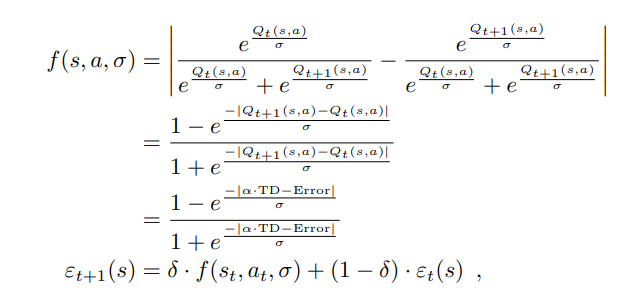
\includegraphics[width=0.8\linewidth]{theory/VDBE_epsilon.png}
            \caption{\label{fig:VDBE_epsilon} На $s$ можно не обращать внимания, $a$ -- выбранное на $t$-ом шаге действие, $\sigma$ -- температура: чем выше, тем ближе распределение к равномерному, чем меньше, тем ближе к жадному \cite{tolic_VDBE}}
        \end{figure}
        \item Epsilon-BMC. Пока не разобрался.
    \end{enumerate}
    В \href{https://en.wikipedia.org/wiki/Multi-armed_bandit}{Википедии} также описаны эти стратегии
    \item Если знаем, какому семейству распределений принадлежат рычаги, то можно для матожиданий и дисперсии в первых двух алгоритмах использовать границы (например) $95\%$-го доверительного интервала.
\end{enumerate}

\subsection{Optimistic initialization}
Можно инициализировать начальные значения всех рычагов большим положительным числом, как и в обычной оптимистичной инициализации. Изменять матожидание можно как среднее арифметическое, так и скользящим окном: $Q_{t+1}(a) = Q_t(a) + \alpha (R_t - Q_t(a))$.

Аналогично с $\overline{R_{t+1}^2(a)}$: $\overline{R_{t+1}^2(a)} = \overline{R_{t}^2(a)} + \alpha (R_t^2 - \overline{R_{t}^2(a)})$.

Выборочная дисперсия изменяется по формуле \ref{eq:1}. Но думаю, что оптимистичная инициализация с const step-size будет работать плохо, как и в обычной задаче о многоруких бандитах.

\subsection{UCB}
Можно ввести UCB для приближения, которое строится, исходя из выбранных ранее рычагов (\ref{subsubsec:iterative_greedy_changing_two_probs}). То есть, аналогично классическому UCB, $A_t = \underset{a}{\arg \max} \left( Q_t(a) - 2 \lambda p_a S_t^2(a) + c \sqrt{\frac{\ln t}{N_t(a)}} \right)$, где $p_a = \frac{N_t(a)}{t-1}$.

Можно еще пытаться что-то проделать с софтмаксом ($H_t(a)$ зависит от $Q_t(a), \, S_t^2(a), \, t, \, N_t(a)$, и $p_a = \frac{e^{H_t(a)}}{\sum_{i=1}^n e^{H_t(i)}}$). Но вот здесь уже меньше уверенности, что сработает.

\subsection{Gradient bandits}

Проводя аналогичные вычисления, что и в параграфе из книги ``Reinforcement Learning: An Inrtroduction'' \cite{suttonbarto_gradient_bandits}, получаем:
\[
    H_{t+1}(a) = H_t(a) + \alpha \frac{\partial \mathbb{E}(Q_{t,p} - \lambda S_{t,p}^2)}{\partial H_t(a)}
\]
\begin{dmath}
    \frac{\partial \mathbb{E}(m_{\pi} - \lambda \sigma_{\pi}^2)}{\partial H_t(a)} = \sum_{x} \left( m_x - 2 \lambda \pi_t(x) \sigma_x^2 \right) \frac{\partial \pi_t(x)}{\partial H_t(a)} = \mathbb{E} \left( \frac{m_{A_t}}{\pi_t(A_t)} - 2 \lambda \sigma_{A_t}^2 - B_t \right) \frac{\partial \pi_t(A_t)}{\partial H_t(a)} = \mathbb{E} \left( m_{A_t} - 2 \lambda \pi_t(A_t) \sigma_{A_t}^2 - B_t \right) \left( \mathbb{I}_{a=A_t} - \pi_t(a) \right) = \mathbb{E} \left( R_t  - 2 \lambda \pi_t(A_t) S_{t+1}^2 (A_t) - B_t \right) \left( \mathbb{I}_{a=A_t} - \pi_t(a) \right) = \mathbb{E} \left( R_t  - 2 \lambda \pi_t(A_t) \frac{N_t(A_t) \overline{R_t^2(A_t)} - 2Q_t(A_t)R_t + R_t^2}{N_t(A_t) + 1} - B_t \right) \left( \mathbb{I}_{a=A_t} - \pi_t(a) \right)
\end{dmath}
Осталось выбрать baseline. Пусть $\overline{R_t^k} = \frac{\sum_{i=1}^{t-1} R_i^k}{t - 1}$, тогда возьмем
\[
\text{baseline} = \overline{R_t} - 2 \lambda \pi_t(A_t) \frac{N_t(A_t) \overline{R_t^2(A_t)} - 2Q_t(A_t) \overline{R_t} + \overline{R_t^2}}{N_t(A_t) + 1}
\]
так как $\forall k \; \mathbb{E} R_k^i = \mathbb{E} R_t^i$.
Итоговая формула:
\begin{dmath}
    H_{t+1}(a) = H_t(a) + \alpha \left[ R_t  - 2 \lambda \pi_t(A_t) \frac{N_t(A_t) \overline{R_t^2(A_t)} - 2Q_t(A_t)R_t + R_t^2}{N_t(A_t) + 1} - \overline{R_t} + 2 \lambda \pi_t(A_t) \frac{N_t(A_t) \overline{R_t^2(A_t)} - 2Q_t(A_t) \overline{R_t} + \overline{R_t^2}}{N_t(A_t) + 1} \right] \left( \mathbb{I}_{a=A_t} - \pi_t(a) \right) = H_t(a) + \alpha \left[ \left(1 - \frac{4 \lambda \pi_t(A_t) Q_t(A_t)}{N_t(A_t) + 1}\right) (R_t - \overline{R_t}) + \frac{2 \lambda \pi_t(A_t)}{N_t(A_t) + 1} (R_t^2 - \overline{R_t^2})\right] \left( \mathbb{I}_{a=A_t} - \pi_t(a) \right)
\end{dmath}
Подсчет суммарно всех $H_{t+1}(a)$ происходит за $O(1)$, если знаем $Q_t(A_t)$ и $N_t(A_t)$.

\subsection{Сэмплирование Томпсона}

Если нам известно, из какого семейства распределений взяты распределения для рычагов (например, из распределения Стьюдента с 3 степенями свободы), то в некоторых случаях можно найти сопряженное семейство распределений. Тогда для обычной задачи о многоруких бандитах можно использовать алгоритм, известный как сэмплирование Томпсона \cite{intro_bandits}: можно считать, что параметры исходного семейства распределений были взяты, исходя из сопряженного семейства распределений. В таком случае, хоть нам и неизвестны исходные параметры, но мы можем оценить их апостериорную вероятность. Исходный алгоритм выглядит так:
\begin{enumerate}
    \item Для каждого рычага сэмплируются матожидания в соответствии своим апостериорным вероятностям
    \item Выбирается рычаг с максимальным сэмплированным матожиданием
    \item Для выбранного рычага выдается награда и обновляются параметры для распределения из сопряженного семейства распределений, соответствующего этому рычагу. Тем самым изменяется представление о том, чему равно матожидание для выбранного рычага.
    \item Возврат к шагу 1.
\end{enumerate}
Сэмплирование Томпсона обладает весомым достоинством -- оно очень быстро находит рычаг с наибольшим матожиданием. А именно: матожидание сожаления $\mathbb{E} \: \overline{\text{Regret}_T} = O\left(\sqrt{n \frac{\log T}{T}} \right)$. Это значительный результат, поскольку, например, для любой стратегии с неадаптивным (то есть не зависящим от истории наград) исследованием при фиксированных $T, n$ существуют распределения на рычагах, при которых  $\mathbb{E} \: \overline{\text{Regret}_T} \geq \Omega \left(n^{1/3} \, T^{-1/3} \right)$ \cite{intro_bandits_slow_convergence}.

Сэмплирование Томпосна можно обобщить для случаев, когда выбор рычага не детерминирован. Рассмотрим такую модификацию для нашей задачи:
\begin{enumerate}
    \item Для каждого рычага сэмплируются матожидания и дисперсии в соответствии своим апостериорным вероятностям
    \item С помощью градиентного подъема или алгоритма за $O(n \log n)$ для выбранных матожиданий и дисперсий находится $P^* = \underset{P \in Q}{\arg \max} (m_P - \lambda \sigma_P^2)$
    \item Выбирается рычаг в соответствии с $P^*$.
    \item Для выбранного рычага выдается награда и обновляются параметры для распределения из сопряженного семейства распределений, соответствующего этому рычагу. Тем самым изменяется представление о том, чему равны матожидание и дсиперсия для выбранного рычага.
    \item Возврат к шагу 1.
\end{enumerate}

Возможно, это не будет работать, но попробовать стоит.
\fi
%% Chapter 1

\chapter{Chapter Title Here} % Main chapter title

\label{Chapter1} % For referencing the chapter elsewhere, use \ref{Chapter1} 

%----------------------------------------------------------------------------------------

% Define some commands to keep the formatting separated from the content 
\newcommand{\keyword}[1]{\textbf{#1}}
\newcommand{\tabhead}[1]{\textbf{#1}}
\newcommand{\code}[1]{\texttt{#1}}
\newcommand{\file}[1]{\texttt{\bfseries#1}}
\newcommand{\option}[1]{\texttt{\itshape#1}}

%----------------------------------------------------------------------------------------

\section{Welcome and Thank You}
Welcome to this \LaTeX{} Thesis Template, a beautiful and easy to use template for writing a thesis using the \LaTeX{} typesetting system.

If you are writing a thesis (or will be in the future) and its subject is technical or mathematical (though it doesn't have to be), then creating it in \LaTeX{} is highly recommended as a way to make sure you can just get down to the essential writing without having to worry over formatting or wasting time arguing with your word processor.

\LaTeX{} is easily able to professionally typeset documents that run to hundreds or thousands of pages long. With simple mark-up commands, it automatically sets out the table of contents, margins, page headers and footers and keeps the formatting consistent and beautiful. One of its main strengths is the way it can easily typeset mathematics, even \emph{heavy} mathematics. Even if those equations are the most horribly twisted and most difficult mathematical problems that can only be solved on a super-computer, you can at least count on \LaTeX{} to make them look stunning.

%----------------------------------------------------------------------------------------

\section{Learning \LaTeX{}}

\LaTeX{} is not a \textsc{wysiwyg} (What You See is What You Get) program, unlike word processors such as Microsoft Word or Apple's Pages. Instead, a document written for \LaTeX{} is actually a simple, plain text file that contains \emph{no formatting}. You tell \LaTeX{} how you want the formatting in the finished document by writing in simple commands amongst the text, for example, if I want to use \emph{italic text for emphasis}, I write the \verb|\emph{text}| command and put the text I want in italics in between the curly braces. This means that \LaTeX{} is a \enquote{mark-up} language, very much like HTML.

\subsection{A (not so short) Introduction to \LaTeX{}}

If you are new to \LaTeX{}, there is a very good eBook -- freely available online as a PDF file -- called, \enquote{The Not So Short Introduction to \LaTeX{}}. The book's title is typically shortened to just \emph{lshort}. You can download the latest version (as it is occasionally updated) from here:
\url{http://www.ctan.org/tex-archive/info/lshort/english/lshort.pdf}

It is also available in several other languages. Find yours from the list on this page: \url{http://www.ctan.org/tex-archive/info/lshort/}

It is recommended to take a little time out to learn how to use \LaTeX{} by creating several, small `test' documents, or having a close look at several templates on:\\ 
\url{http://www.LaTeXTemplates.com}\\ 
Making the effort now means you're not stuck learning the system when what you \emph{really} need to be doing is writing your thesis.

\subsection{A Short Math Guide for \LaTeX{}}

If you are writing a technical or mathematical thesis, then you may want to read the document by the AMS (American Mathematical Society) called, \enquote{A Short Math Guide for \LaTeX{}}. It can be found online here:
\url{http://www.ams.org/tex/amslatex.html}
under the \enquote{Additional Documentation} section towards the bottom of the page.

\subsection{Common \LaTeX{} Math Symbols}
There are a multitude of mathematical symbols available for \LaTeX{} and it would take a great effort to learn the commands for them all. The most common ones you are likely to use are shown on this page:
\url{http://www.sunilpatel.co.uk/latex-type/latex-math-symbols/}

You can use this page as a reference or crib sheet, the symbols are rendered as large, high quality images so you can quickly find the \LaTeX{} command for the symbol you need.

\subsection{\LaTeX{} on a Mac}
 
The \LaTeX{} distribution is available for many systems including Windows, Linux and Mac OS X. The package for OS X is called MacTeX and it contains all the applications you need -- bundled together and pre-customized -- for a fully working \LaTeX{} environment and work flow.
 
MacTeX includes a custom dedicated \LaTeX{} editor called TeXShop for writing your `\file{.tex}' files and BibDesk: a program to manage your references and create your bibliography section just as easily as managing songs and creating playlists in iTunes.

%----------------------------------------------------------------------------------------

\section{Getting Started with this Template}

If you are familiar with \LaTeX{}, then you should explore the directory structure of the template and then proceed to place your own information into the \emph{THESIS INFORMATION} block of the \file{main.tex} file. You can then modify the rest of this file to your unique specifications based on your degree/university. Section \ref{FillingFile} on page \pageref{FillingFile} will help you do this. Make sure you also read section \ref{ThesisConventions} about thesis conventions to get the most out of this template.

If you are new to \LaTeX{} it is recommended that you carry on reading through the rest of the information in this document.

Before you begin using this template you should ensure that its style complies with the thesis style guidelines imposed by your institution. In most cases this template style and layout will be suitable. If it is not, it may only require a small change to bring the template in line with your institution's recommendations. These modifications will need to be done on the \file{MastersDoctoralThesis.cls} file.

\subsection{About this Template}

This \LaTeX{} Thesis Template is originally based and created around a \LaTeX{} style file created by Steve R.\ Gunn from the University of Southampton (UK), department of Electronics and Computer Science. You can find his original thesis style file at his site, here:
\url{http://www.ecs.soton.ac.uk/~srg/softwaretools/document/templates/}

Steve's \file{ecsthesis.cls} was then taken by Sunil Patel who modified it by creating a skeleton framework and folder structure to place the thesis files in. The resulting template can be found on Sunil's site here:
\url{http://www.sunilpatel.co.uk/thesis-template}

Sunil's template was made available through \url{http://www.LaTeXTemplates.com} where it was modified many times based on user requests and questions. Version 2.0 and onwards of this template represents a major modification to Sunil's template and is, in fact, hardly recognisable. The work to make version 2.0 possible was carried out by \href{mailto:vel@latextemplates.com}{Vel} and Johannes Böttcher.

%----------------------------------------------------------------------------------------

\section{What this Template Includes}

\subsection{Folders}

This template comes as a single zip file that expands out to several files and folders. The folder names are mostly self-explanatory:

\keyword{Appendices} -- this is the folder where you put the appendices. Each appendix should go into its own separate \file{.tex} file. An example and template are included in the directory.

\keyword{Chapters} -- this is the folder where you put the thesis chapters. A thesis usually has about six chapters, though there is no hard rule on this. Each chapter should go in its own separate \file{.tex} file and they can be split as:
\begin{itemize}
\item Chapter 1: Introduction to the thesis topic
\item Chapter 2: Background information and theory
\item Chapter 3: (Laboratory) experimental setup
\item Chapter 4: Details of experiment 1
\item Chapter 5: Details of experiment 2
\item Chapter 6: Discussion of the experimental results
\item Chapter 7: Conclusion and future directions
\end{itemize}
This chapter layout is specialised for the experimental sciences, your discipline may be different.

\keyword{Figures} -- this folder contains all figures for the thesis. These are the final images that will go into the thesis document.

\subsection{Files}

Included are also several files, most of them are plain text and you can see their contents in a text editor. After initial compilation, you will see that more auxiliary files are created by \LaTeX{} or BibTeX and which you don't need to delete or worry about:

\keyword{example.bib} -- this is an important file that contains all the bibliographic information and references that you will be citing in the thesis for use with BibTeX. You can write it manually, but there are reference manager programs available that will create and manage it for you. Bibliographies in \LaTeX{} are a large subject and you may need to read about BibTeX before starting with this. Many modern reference managers will allow you to export your references in BibTeX format which greatly eases the amount of work you have to do.

\keyword{MastersDoctoralThesis.cls} -- this is an important file. It is the class file that tells \LaTeX{} how to format the thesis. 

\keyword{main.pdf} -- this is your beautifully typeset thesis (in the PDF file format) created by \LaTeX{}. It is supplied in the PDF with the template and after you compile the template you should get an identical version.

\keyword{main.tex} -- this is an important file. This is the file that you tell \LaTeX{} to compile to produce your thesis as a PDF file. It contains the framework and constructs that tell \LaTeX{} how to layout the thesis. It is heavily commented so you can read exactly what each line of code does and why it is there. After you put your own information into the \emph{THESIS INFORMATION} block -- you have now started your thesis!

Files that are \emph{not} included, but are created by \LaTeX{} as auxiliary files include:

\keyword{main.aux} -- this is an auxiliary file generated by \LaTeX{}, if it is deleted \LaTeX{} simply regenerates it when you run the main \file{.tex} file.

\keyword{main.bbl} -- this is an auxiliary file generated by BibTeX, if it is deleted, BibTeX simply regenerates it when you run the \file{main.aux} file. Whereas the \file{.bib} file contains all the references you have, this \file{.bbl} file contains the references you have actually cited in the thesis and is used to build the bibliography section of the thesis.

\keyword{main.blg} -- this is an auxiliary file generated by BibTeX, if it is deleted BibTeX simply regenerates it when you run the main \file{.aux} file.

\keyword{main.lof} -- this is an auxiliary file generated by \LaTeX{}, if it is deleted \LaTeX{} simply regenerates it when you run the main \file{.tex} file. It tells \LaTeX{} how to build the \emph{List of Figures} section.

\keyword{main.log} -- this is an auxiliary file generated by \LaTeX{}, if it is deleted \LaTeX{} simply regenerates it when you run the main \file{.tex} file. It contains messages from \LaTeX{}, if you receive errors and warnings from \LaTeX{}, they will be in this \file{.log} file.

\keyword{main.lot} -- this is an auxiliary file generated by \LaTeX{}, if it is deleted \LaTeX{} simply regenerates it when you run the main \file{.tex} file. It tells \LaTeX{} how to build the \emph{List of Tables} section.

\keyword{main.out} -- this is an auxiliary file generated by \LaTeX{}, if it is deleted \LaTeX{} simply regenerates it when you run the main \file{.tex} file.

So from this long list, only the files with the \file{.bib}, \file{.cls} and \file{.tex} extensions are the most important ones. The other auxiliary files can be ignored or deleted as \LaTeX{} and BibTeX will regenerate them.

%----------------------------------------------------------------------------------------

\section{Filling in Your Information in the \file{main.tex} File}\label{FillingFile}

You will need to personalise the thesis template and make it your own by filling in your own information. This is done by editing the \file{main.tex} file in a text editor or your favourite LaTeX environment.

Open the file and scroll down to the third large block titled \emph{THESIS INFORMATION} where you can see the entries for \emph{University Name}, \emph{Department Name}, etc \ldots

Fill out the information about yourself, your group and institution. You can also insert web links, if you do, make sure you use the full URL, including the \code{http://} for this. If you don't want these to be linked, simply remove the \verb|\href{url}{name}| and only leave the name.

When you have done this, save the file and recompile \code{main.tex}. All the information you filled in should now be in the PDF, complete with web links. You can now begin your thesis proper!

%----------------------------------------------------------------------------------------

\section{The \code{main.tex} File Explained}

The \file{main.tex} file contains the structure of the thesis. There are plenty of written comments that explain what pages, sections and formatting the \LaTeX{} code is creating. Each major document element is divided into commented blocks with titles in all capitals to make it obvious what the following bit of code is doing. Initially there seems to be a lot of \LaTeX{} code, but this is all formatting, and it has all been taken care of so you don't have to do it.

Begin by checking that your information on the title page is correct. For the thesis declaration, your institution may insist on something different than the text given. If this is the case, just replace what you see with what is required in the \emph{DECLARATION PAGE} block.

Then comes a page which contains a funny quote. You can put your own, or quote your favourite scientist, author, person, and so on. Make sure to put the name of the person who you took the quote from.

Following this is the abstract page which summarises your work in a condensed way and can almost be used as a standalone document to describe what you have done. The text you write will cause the heading to move up so don't worry about running out of space.

Next come the acknowledgements. On this page, write about all the people who you wish to thank (not forgetting parents, partners and your advisor/supervisor).

The contents pages, list of figures and tables are all taken care of for you and do not need to be manually created or edited. The next set of pages are more likely to be optional and can be deleted since they are for a more technical thesis: insert a list of abbreviations you have used in the thesis, then a list of the physical constants and numbers you refer to and finally, a list of mathematical symbols used in any formulae. Making the effort to fill these tables means the reader has a one-stop place to refer to instead of searching the internet and references to try and find out what you meant by certain abbreviations or symbols.

The list of symbols is split into the Roman and Greek alphabets. Whereas the abbreviations and symbols ought to be listed in alphabetical order (and this is \emph{not} done automatically for you) the list of physical constants should be grouped into similar themes.

The next page contains a one line dedication. Who will you dedicate your thesis to?

Finally, there is the block where the chapters are included. Uncomment the lines (delete the \code{\%} character) as you write the chapters. Each chapter should be written in its own file and put into the \emph{Chapters} folder and named \file{Chapter1}, \file{Chapter2}, etc\ldots Similarly for the appendices, uncomment the lines as you need them. Each appendix should go into its own file and placed in the \emph{Appendices} folder.

After the preamble, chapters and appendices finally comes the bibliography. The bibliography style (called \option{authoryear}) is used for the bibliography and is a fully featured style that will even include links to where the referenced paper can be found online. Do not underestimate how grateful your reader will be to find that a reference to a paper is just a click away. Of course, this relies on you putting the URL information into the BibTeX file in the first place.

%----------------------------------------------------------------------------------------

\section{Thesis Features and Conventions}\label{ThesisConventions}

To get the best out of this template, there are a few conventions that you may want to follow.

One of the most important (and most difficult) things to keep track of in such a long document as a thesis is consistency. Using certain conventions and ways of doing things (such as using a Todo list) makes the job easier. Of course, all of these are optional and you can adopt your own method.

\subsection{Printing Format}

This thesis template is designed for double sided printing (i.e. content on the front and back of pages) as most theses are printed and bound this way. Switching to one sided printing is as simple as uncommenting the \option{oneside} option of the \code{documentclass} command at the top of the \file{main.tex} file. You may then wish to adjust the margins to suit specifications from your institution.

The headers for the pages contain the page number on the outer side (so it is easy to flick through to the page you want) and the chapter name on the inner side.

The text is set to 11 point by default with single line spacing, again, you can tune the text size and spacing should you want or need to using the options at the very start of \file{main.tex}. The spacing can be changed similarly by replacing the \option{singlespacing} with \option{onehalfspacing} or \option{doublespacing}.

\subsection{Using US Letter Paper}

The paper size used in the template is A4, which is the standard size in Europe. If you are using this thesis template elsewhere and particularly in the United States, then you may have to change the A4 paper size to the US Letter size. This can be done in the margins settings section in \file{main.tex}.

Due to the differences in the paper size, the resulting margins may be different to what you like or require (as it is common for institutions to dictate certain margin sizes). If this is the case, then the margin sizes can be tweaked by modifying the values in the same block as where you set the paper size. Now your document should be set up for US Letter paper size with suitable margins.

\subsection{References}

The \code{biblatex} package is used to format the bibliography and inserts references such as this one \parencite{Reference1}. The options used in the \file{main.tex} file mean that the in-text citations of references are formatted with the author(s) listed with the date of the publication. Multiple references are separated by semicolons (e.g. \parencite{Reference2, Reference1}) and references with more than three authors only show the first author with \emph{et al.} indicating there are more authors (e.g. \parencite{Reference3}). This is done automatically for you. To see how you use references, have a look at the \file{Chapter1.tex} source file. Many reference managers allow you to simply drag the reference into the document as you type.

Scientific references should come \emph{before} the punctuation mark if there is one (such as a comma or period). The same goes for footnotes\footnote{Such as this footnote, here down at the bottom of the page.}. You can change this but the most important thing is to keep the convention consistent throughout the thesis. Footnotes themselves should be full, descriptive sentences (beginning with a capital letter and ending with a full stop). The APA6 states: \enquote{Footnote numbers should be superscripted, [...], following any punctuation mark except a dash.} The Chicago manual of style states: \enquote{A note number should be placed at the end of a sentence or clause. The number follows any punctuation mark except the dash, which it precedes. It follows a closing parenthesis.}

The bibliography is typeset with references listed in alphabetical order by the first author's last name. This is similar to the APA referencing style. To see how \LaTeX{} typesets the bibliography, have a look at the very end of this document (or just click on the reference number links in in-text citations).

\subsubsection{A Note on bibtex}

The bibtex backend used in the template by default does not correctly handle unicode character encoding (i.e. "international" characters). You may see a warning about this in the compilation log and, if your references contain unicode characters, they may not show up correctly or at all. The solution to this is to use the biber backend instead of the outdated bibtex backend. This is done by finding this in \file{main.tex}: \option{backend=bibtex} and changing it to \option{backend=biber}. You will then need to delete all auxiliary BibTeX files and navigate to the template directory in your terminal (command prompt). Once there, simply type \code{biber main} and biber will compile your bibliography. You can then compile \file{main.tex} as normal and your bibliography will be updated. An alternative is to set up your LaTeX editor to compile with biber instead of bibtex, see \href{http://tex.stackexchange.com/questions/154751/biblatex-with-biber-configuring-my-editor-to-avoid-undefined-citations/}{here} for how to do this for various editors.

\subsection{Tables}

Tables are an important way of displaying your results, below is an example table which was generated with this code:

{\small
\begin{verbatim}
\begin{table}
\caption{The effects of treatments X and Y on the four groups studied.}
\label{tab:treatments}
\centering
\begin{tabular}{l l l}
\toprule
\tabhead{Groups} & \tabhead{Treatment X} & \tabhead{Treatment Y} \\
\midrule
1 & 0.2 & 0.8\\
2 & 0.17 & 0.7\\
3 & 0.24 & 0.75\\
4 & 0.68 & 0.3\\
\bottomrule\\
\end{tabular}
\end{table}
\end{verbatim}
}

\begin{table}
\caption{The effects of treatments X and Y on the four groups studied.}
\label{tab:treatments}
\centering
\begin{tabular}{l l l}
\toprule
\tabhead{Groups} & \tabhead{Treatment X} & \tabhead{Treatment Y} \\
\midrule
1 & 0.2 & 0.8\\
2 & 0.17 & 0.7\\
3 & 0.24 & 0.75\\
4 & 0.68 & 0.3\\
\bottomrule\\
\end{tabular}
\end{table}

You can reference tables with \verb|\ref{<label>}| where the label is defined within the table environment. See \file{Chapter1.tex} for an example of the label and citation (e.g. Table~\ref{tab:treatments}).

\subsection{Figures}

There will hopefully be many figures in your thesis (that should be placed in the \emph{Figures} folder). The way to insert figures into your thesis is to use a code template like this:
\begin{verbatim}
\begin{figure}
\centering

\includegraphics{Figures/Electron}
\decoRule
\caption[An Electron]{An electron (artist's impression).}
\label{fig:Electron}
\end{figure}
\end{verbatim}
Also look in the source file. Putting this code into the source file produces the picture of the electron that you can see in the figure below.

\begin{figure}[th]
\centering

\includegraphics{Figures/Electron}
\decoRule
\caption[An Electron]{An electron (artist's impression).}
\label{fig:Electron}
\end{figure}

Sometimes figures don't always appear where you write them in the source. The placement depends on how much space there is on the page for the figure. Sometimes there is not enough room to fit a figure directly where it should go (in relation to the text) and so \LaTeX{} puts it at the top of the next page. Positioning figures is the job of \LaTeX{} and so you should only worry about making them look good!

Figures usually should have captions just in case you need to refer to them (such as in Figure~\ref{fig:Electron}). The \verb|\caption| command contains two parts, the first part, inside the square brackets is the title that will appear in the \emph{List of Figures}, and so should be short. The second part in the curly brackets should contain the longer and more descriptive caption text.

The \verb|\decoRule| command is optional and simply puts an aesthetic horizontal line below the image. If you do this for one image, do it for all of them.

\LaTeX{} is capable of using images in pdf, jpg and png format.

\subsection{Typesetting mathematics}

If your thesis is going to contain heavy mathematical content, be sure that \LaTeX{} will make it look beautiful, even though it won't be able to solve the equations for you.

The \enquote{Not So Short Introduction to \LaTeX} (available on \href{http://www.ctan.org/tex-archive/info/lshort/english/lshort.pdf}{CTAN}) should tell you everything you need to know for most cases of typesetting mathematics. If you need more information, a much more thorough mathematical guide is available from the AMS called, \enquote{A Short Math Guide to \LaTeX} and can be downloaded from:
\url{ftp://ftp.ams.org/pub/tex/doc/amsmath/short-math-guide.pdf}

There are many different \LaTeX{} symbols to remember, luckily you can find the most common symbols in \href{http://ctan.org/pkg/comprehensive}{The Comprehensive \LaTeX~Symbol List}.

You can write an equation, which is automatically given an equation number by \LaTeX{} like this:
\begin{verbatim}
\begin{equation}
E = mc^{2}
\label{eqn:Einstein}
\end{equation}
\end{verbatim}

This will produce Einstein's famous energy-matter equivalence equation:
\begin{equation}
E = mc^{2}
\label{eqn:Einstein}
\end{equation}

All equations you write (which are not in the middle of paragraph text) are automatically given equation numbers by \LaTeX{}. If you don't want a particular equation numbered, use the unnumbered form:
\begin{verbatim}
\[ a^{2}=4 \]
\end{verbatim}

%----------------------------------------------------------------------------------------

\section{Sectioning and Subsectioning}

You should break your thesis up into nice, bite-sized sections and subsections. \LaTeX{} automatically builds a table of Contents by looking at all the \verb|\chapter{}|, \verb|\section{}|  and \verb|\subsection{}| commands you write in the source.

The Table of Contents should only list the sections to three (3) levels. A \verb|chapter{}| is level zero (0). A \verb|\section{}| is level one (1) and so a \verb|\subsection{}| is level two (2). In your thesis it is likely that you will even use a \verb|subsubsection{}|, which is level three (3). The depth to which the Table of Contents is formatted is set within \file{MastersDoctoralThesis.cls}. If you need this changed, you can do it in \file{main.tex}.

%----------------------------------------------------------------------------------------

\section{In Closing}

You have reached the end of this mini-guide. You can now rename or overwrite this pdf file and begin writing your own \file{Chapter1.tex} and the rest of your thesis. The easy work of setting up the structure and framework has been taken care of for you. It's now your job to fill it out!

Good luck and have lots of fun!

\begin{flushright}
Guide written by ---\\
Sunil Patel: \href{http://www.sunilpatel.co.uk}{www.sunilpatel.co.uk}\\
Vel: \href{http://www.LaTeXTemplates.com}{LaTeXTemplates.com}
\end{flushright}

%\include{Chapters/Chapter2} 
%\include{Chapters/Chapter3}
%\include{Chapters/Chapter4} 
%\include{Chapters/Chapter5} 

%----------------------------------------------------------------------------------------
%	THESIS CONTENT - APPENDICES
%----------------------------------------------------------------------------------------

\appendix % Cue to tell LaTeX that the following "chapters" are Appendices

% Include the appendices of the thesis as separate files from the Appendices folder
% Uncomment the lines as you write the Appendices

% Appendix A

\chapter{Frequently Asked Questions} % Main appendix title

\label{AppendixA} % For referencing this appendix elsewhere, use \ref{AppendixA}

\section{How do I change the colors of links?}

The color of links can be changed to your liking using:

{\small\verb!\hypersetup{urlcolor=red}!}, or

{\small\verb!\hypersetup{citecolor=green}!}, or

{\small\verb!\hypersetup{allcolor=blue}!}.

\noindent If you want to completely hide the links, you can use:

{\small\verb!\hypersetup{allcolors=.}!}, or even better: 

{\small\verb!\hypersetup{hidelinks}!}.

\noindent If you want to have obvious links in the PDF but not the printed text, use:

{\small\verb!\hypersetup{colorlinks=false}!}.

%\include{Appendices/AppendixB}
%\include{Appendices/AppendixC}

%----------------------------------------------------------------------------------------
%	BIBLIOGRAPHY
%----------------------------------------------------------------------------------------

\printbibliography[heading=bibintoc]

%----------------------------------------------------------------------------------------

%----------------------------------------------------------------------------------------
%	ACKNOWLEDGEMENTS
%----------------------------------------------------------------------------------------

% Remove this page if you do not want to add any acknowledgements

\begin{acknowledgements}
	\addchaptertocentry{\acknowledgementname} % Add the acknowledgements to the table of contents
	The acknowledgments and the people to thank go here, don't forget to include your project advisor\ldots
\end{acknowledgements}

\end{document}  
